\documentclass{wlscirep}
\usepackage[utf8]{inputenc}
\usepackage[T1]{fontenc}
\usepackage{booktabs}
\usepackage{multirow}
\usepackage{graphicx}
\usepackage{amsmath}
\usepackage{amssymb}
\usepackage{xcolor}
\usepackage{url}
\usepackage{tabularx}
\usepackage{adjustbox}
\usepackage{float}
\usepackage{pifont}
\usepackage[normalem]{ulem}
\usepackage[outerbars]{changebar}
\usepackage{lineno}


\definecolor{correct}{RGB}{0,100,200}
\definecolor{incorrect}{RGB}{220,38,38}
\definecolor{hallucinated}{RGB}{22,163,74}

%% ─────────────────────────────────────────────────────────────────
%% Разметка правок ревизии.
%%   \markupfalse — чистая рукопись (файл для основной подачи);
%%   \markuptrue  — подсвеченная версия (marked-up, в related files).
%% Обе версии собираются из ЭТОГО файла: переключается одна строка ниже,
%% ничего больше править не нужно.
%% ─────────────────────────────────────────────────────────────────
\newif\ifmarkup
% Подсвеченная версия собирается БЕЗ правки этого файла: в Overleaf нужно
% выбрать главным документом main_marked.tex — он задаёт \MARKUPVERSION
% и подключает этот же файл. Так обе версии всегда остаются синхронными.
\ifdefined\MARKUPVERSION \markuptrue \else \markupfalse \fi

\definecolor{revised}{RGB}{0,90,160}
\definecolor{markerbar}{RGB}{240,170,20}
\cbcolor{markerbar}
\setlength{\changebarwidth}{3pt}
\setlength{\changebarsep}{6pt}
% \rev{...}    — новый или переписанный текст
% \del{...}    — удалённый короткий фрагмент (зачёркивание); ТОЛЬКО вне формул,
%                \sout несовместим с математическим режимом
% \delpar{...} — удалённый крупный фрагмент (без зачёркивания: \sout ломается
%                на длинных абзацах с \cite, а проверить сборку локально нельзя)
% Тексты внутри макросов только латиницей: преамбула использует [T1]{fontenc},
% в котором нет кириллицы.
%% Стиль разметки правок:
%%   \markbartrue  — текст остаётся ЧЁРНЫМ, правка отмечается цветной полосой
%%                   на поле (как отчерк маркером). Работает с формулами,
%%                   ссылками и фрагментами длиннее абзаца;
%%   \markbarfalse — правка выделяется синим текстом.
%% Внутри таблиц и рисунков полосу на поле LaTeX не рисует (ограничение
%% плавающих объектов), поэтому там всегда используется цвет — макросы
%% \revf и \revmf.
\newif\ifmarkbar
\markbartrue

\newcommand{\rev}[1]{%
  \ifmarkup
    \ifmarkbar\cbstart#1\cbend\else\textcolor{revised}{#1}\fi
  \else#1\fi}
% \revm{...} — то же для содержимого формул: \textcolor опирается на \leavevmode
%              и в математическом режиме ненадёжен, \color безопасен
\newcommand{\revm}[1]{\ifmarkup\ifmarkbar#1\else{\color{revised}#1}\fi\else#1\fi}
% \revf / \revmf — внутри плавающих объектов: только цвет
\newcommand{\revf}[1]{\ifmarkup\textcolor{revised}{#1}\else#1\fi}
\newcommand{\revmf}[1]{\ifmarkup{\color{revised}#1}\else#1\fi}
\newcommand{\del}[1]{\ifmarkup\textcolor{incorrect}{\sout{#1}}\fi}
\newcommand{\delpar}[1]{\ifmarkup\textcolor{incorrect}{[\textbf{REMOVED:} #1]}\fi}
% \todo{...} — незаполненный слот. Печатается ВСЕГДА, в том числе в чистой версии:
% это защита от подачи с незаполненными данными, а не пометка для себя.
\newcommand{\todo}[1]{\textcolor{incorrect}{\textbf{[TODO: #1]}}}

\title{Two-Stage Synthetic-to-Real Transfer Learning for Automated Mammography Report Generation Using Vision-Language Models}

\author[1]{Gani Esen}
\author[1,2,*]{Marat Nurtas}
\author[3]{Jandos Amankulov}
\author[4]{Laura La Paglia}

\affil[1]{Faculty of Information Technology, International Information Technology University, Almaty 050000, Kazakhstan} 
\affil[2] {Faculty of Information Technology and Artificial Intelligence, Al-Farabi Kazakh National University,  Almaty 050000, Kazakhstan}
\affil[3]{Department of Radiology and Nuclear Medicine, Kazakh Institute of Oncology and Radiology, Almaty 050051, Kazakhstan}
\affil[4]{Institute for High Performance Computing and Networking (ICAR), National Research Council (CNR) of Italy, Via Ugo La Malfa 153, Palermo 90146, Italy}
\affil[*]{Corresponding author: m.nurtas@iitu.edu.kz}

\keywords{mammography; report generation; vision-language models; low-rank adaptation; equivalence testing; negative result}

%% ─────────────────────────────────────────────────────────────────
%% Абстракт переписан 08.08.2026 под фактические результаты ревизии:
%% сняты «clinically validated», заявление о 2x экономии данных и снижение
%% галлюцинаций 73.1% → 21.2%; «nine» → «eight»; BERTScore 0.917 → 0.919
%% (пересчитан одним протоколом). Добавлены главный отрицательный результат
%% (эквивалентность при равной ёмкости на сетке 3x3x3) и расхождение
%% беглости с клинической надёжностью внутри одной модели.
%% ─────────────────────────────────────────────────────────────────

\begin{abstract}
\rev{Automated mammography report generation is constrained by the scarcity of paired mammogram-report data: public collections such as VinDr-Mammo and CBIS-DDSM provide structured annotations but no free-text reports. We propose a two-stage synthetic-to-real framework in which BI-RADS annotations are converted into synthetic reports (400 generated, 390 retained) to pretrain MedGemma-4B with multimodal LoRA, followed by fine-tuning on 407 real DMID reports. It reaches ROUGE-L 0.671, METEOR 0.685, CIDEr 0.729 and BERTScore 0.919 on the DMID test set, exceeding eight baselines and previously reported results. We then test whether synthetic pretraining produces these numbers, and find that it does not: the original advantage was measured between models of unequal adapter capacity, and at matched capacity the two schemes are equivalent. Across 40 training runs over three corpus sizes, capacities and initialisations, against a preset margin, no configuration favours two-stage training; capacity alone reproduces the gap. Two findings bear on evaluation. Under an assertion-level criterion no model fabricates findings; the characteristic error is omission. Textual and clinical quality diverge within one model: where two-stage training gains 0.058 ROUGE-L, BI-RADS agreement and sensitivity both fall. With agreement never exceeding $\kappa = 0.17$, the obstacle to clinically useful reporting is diagnostic accuracy, not fluency.}
\end{abstract}

\begin{document}
\raggedbottom
\maketitle
% Требования Sci Rep к пересмотренной рукописи: арабские номера
% страниц в колонтитуле и номера строк для удобства рецензентов
\thispagestyle{plain}
\pagestyle{plain}
\linenumbers

% Шапка подсвеченной версии. Видна ТОЛЬКО при \markuptrue, поэтому служит
% индикатором: если её нет, значит собирается чистая версия.
\ifmarkup
  \begin{center}
  \fcolorbox{revised}{white}{\parbox{0.93\linewidth}{\small
  \textbf{MARKED-UP COPY.}
  \ifmarkbar
    Text added or rewritten in this revision is marked by a
    \textcolor{markerbar}{\rule{9pt}{3pt}} bar in the outer margin;
    the text itself is unchanged in colour.
    Inside tables and figure captions the margin bar is unavailable, so
    revised text there is shown \textcolor{revised}{in blue} instead.
  \else
    Text added or rewritten in this revision is shown
    \textcolor{revised}{in blue}.
  \fi
  \textcolor{incorrect}{\sout{Deleted text is struck through in red}}
  and larger deletions are summarised as
  \textcolor{incorrect}{[REMOVED: \ldots]}.
  \textcolor{incorrect}{\textbf{[TODO: \ldots]}} marks a slot that is still to be
  filled and appears in both versions.
  The clean manuscript is produced from the same source by compiling
  \texttt{main.tex} instead of \texttt{main\_marked.tex}.}}
  \end{center}
  \vspace{0.6em}
\fi


%% ─────────────────────────────────────────────────────────────────
\section*{Introduction}
%% ─────────────────────────────────────────────────────────────────

Breast cancer remains the most commonly diagnosed cancer worldwide, with approximately 2.3 million new cases in 2022 and representing the leading cause of cancer-related mortality in women~\cite{bray2024global}. Mammography remains the gold standard for population-level breast cancer screening, with evidence demonstrating that regular screening reduces breast cancer mortality by 20--40\% through early-stage detection~\cite{lehman2015mammographic, sechopoulos2021artificial}. However, the clinical utility of mammography is fundamentally constrained by two interrelated challenges: a global shortage of trained radiologists and the high cognitive burden of interpreting large volumes of screening examinations.

Deep learning has shown remarkable success in medical imaging~\cite{esteva2019guide}, including mammography-based cancer detection~\cite{mckinney2020international, lotter2021robust, shen2019deep} and risk prediction~\cite{yala2019deep}. Radiologists are required to produce standardised structured reports following the Breast Imaging Reporting and Data System (BI-RADS) lexicon developed by the American College of Radiology~\cite{birads2013}. These reports must accurately characterise breast density~\cite{gastounioti2022breast, lehman2019mammographic}, describe identified findings (masses, calcifications, architectural distortions, asymmetries), assign a BI-RADS assessment category (0--6), and specify a management recommendation. Report generation is time-intensive, and inter-reader variability remains a persistent limitation. Automated report generation systems that assist radiologists by producing structured report drafts represent a high-value clinical application.

Recent advances in Vision-Language Models (VLMs) have demonstrated remarkable capabilities in generating natural language descriptions from medical images~\cite{wang2024mllm_survey}. Models such as LLaVA-Med~\cite{li2024llavamed}, BiomedCLIP~\cite{zhang2023biomedclip}, and MedGemma~\cite{lin2024medgemma} have shown strong performance on radiology report generation, particularly for chest X-ray interpretation using the MIMIC-CXR dataset~\cite{johnson2019mimiccxr}. Large language models such as Med-PaLM~\cite{singhal2023medpalm} have demonstrated clinical-level knowledge, while Med-Flamingo~\cite{moor2023medflamingo} explored few-shot medical reasoning. However, mammography remains significantly underexplored within the VLM literature. Unlike chest radiography, mammography presents unique challenges: high-resolution full-field digital images requiring fine-grained lesion characterisation, the clinical necessity of multi-view reasoning across craniocaudal (CC) and mediolateral oblique (MLO) projections, and a domain-specific reporting vocabulary governed by the BI-RADS lexicon.

The central obstacle to developing VLMs for mammography report generation is the absence of large-scale publicly available paired datasets---collections of mammographic images matched with corresponding narrative radiology reports. While several public mammography datasets exist, including CBIS-DDSM~\cite{lee2017curated} and VinDr-Mammo~\cite{nguyen2023vindr}, these resources provide structured annotations rather than free-text radiology reports. Only the Digital Mammography Dataset for Breast Cancer Diagnosis Research (DMID)~\cite{oza2024} provides a modest collection (225 cases, 510 images) of paired images and narrative reports; all other publicly accessible mammography datasets lack this critical pairing. Aitimov et al.~\cite{aitimov2025feature} recently developed feature extraction methods for breast cancer detection on VinDr-Mammo using modified Faster R-CNN, demonstrating growing interest in computational mammography from the Central Asian research community.

Our prior work explored dimensionality reduction for breast cancer classification~\cite{esen2024pca}, multi-task attention-guided architectures for joint pathology and density estimation in mammography~\cite{esen2025multitask}, and reinforcement learning with visual interpretability for breast cancer diagnosis~\cite{esen2025rl}. The current work extends this line of research from classification to automated report generation.

To address the data scarcity challenge, we propose a two-stage synthetic-to-real transfer learning framework for automated mammography report generation. Our contributions are:

\begin{enumerate}
    \rev{\item We introduce a \textbf{scalable label-to-report synthesis pipeline} that converts publicly available structured mammography annotations into synthetic training reports, with automated validation of BI-RADS mention, recommendation presence and minimum length. We release the corpus together with an audit of its defects, including 5.4\% of reports generated in the wrong language and passed by the validator.}
    \rev{\item We evaluate the resulting \textbf{two-stage transfer learning framework} against eight baseline methods on the DMID benchmark, spanning zero-shot VLMs, pipeline models and direct fine-tuning, under a single fully specified training and evaluation protocol.}
    \rev{\item We show that \textbf{synthetic pretraining confers no advantage at matched adapter capacity}. Using 40 training runs over three synthetic corpus sizes, three capacities and three initialisations, with an equivalence margin declared in advance, we obtain equivalence or an inconclusive verdict in every cell and superiority in none. We trace the originally reported effect to four measured artefacts, of which the dominant one is a comparison between models of unequal capacity.}
    \rev{\item We provide a \textbf{clinical analysis at matched capacity} showing that these models do not fabricate findings but omit them, that omission affects up to a third of the cases whose reference asserts a finding, and that BI-RADS agreement does not exceed $\kappa = 0.17$ for any model evaluated.}
    \rev{\item We document a \textbf{divergence between textual and clinical quality within a single model}: at small adapter rank two-stage training gains 0.058 ROUGE-L ($p=0.0001$) while losing BI-RADS agreement and finding sensitivity. We argue from this that $n$-gram overlap should not be used to select mammography report generators.}
\end{enumerate}

%% ─────────────────────────────────────────────────────────────────
\section*{Related Work}
%% ─────────────────────────────────────────────────────────────────

\subsection*{Automated Radiology Report Generation}

Automated radiology report generation has been studied extensively for chest X-ray interpretation, where large paired image-report datasets such as MIMIC-CXR~\cite{johnson2019mimiccxr} have enabled supervised learning. Early methods relied on CNN-LSTM architectures with attention mechanisms, while more recent approaches leverage transformer-based~\cite{vaswani2017attention} encoder-decoder frameworks. R2Gen~\cite{chen2020r2gen} introduced a relational memory-driven decoder, while R2GenCMN~\cite{chen2022r2gencmn} extended this with cross-modal memory networks. Miura et al.~\cite{miura2021improving} addressed factual completeness and consistency in report generation. PromptMRG~\cite{jin2024promptmrg} introduced diagnosis-driven prompts for medical report generation. CT2Rep~\cite{hamamci2024ct2rep} extended automated report generation to 3D medical imaging. Despite these advances, mammography remains largely unaddressed due to data scarcity.

\subsection*{Vision-Language Models for Mammography}

Vision-language models such as CLIP~\cite{radford2021clip} and its medical adaptations BiomedCLIP~\cite{zhang2023biomedclip} have enabled multimodal understanding of medical images. LLaVA~\cite{liu2024llava} and its medical variant LLaVA-Med~\cite{li2024llavamed} demonstrated visual instruction tuning for medical question answering.

For mammography specifically, Mammo-CLIP~\cite{ghosh2024} introduced the first VLM pretrained on screening mammogram-report pairs. MV-MLM~\cite{ahmed2025} extended this with multi-view contrastive learning using synthetic text reports. AMRG~\cite{sung2025} established the first reproducible benchmark for mammography report generation, fine-tuning MedGemma-4B with LoRA~\cite{hu2022lora} on the DMID dataset and achieving ROUGE-L of 0.569, METEOR of 0.615, and CIDEr of 0.582, with systematic LoRA hyperparameter exploration across five VLM backbones. MammoWise~\cite{jahangir2026} proposed a local multi-model RAG pipeline with QLoRA~\cite{dettmers2024qlora} fine-tuning achieving BI-RADS accuracy of 0.755. Our work introduces a two-stage training paradigm that surpasses all prior work on the DMID benchmark.

\subsection*{Transfer Learning in Medical Imaging}

Transfer learning from large-scale pretraining to domain-specific fine-tuning has become the dominant paradigm in medical image analysis~\cite{pan2010transfer, zhuang2021survey}. Deep representation learning~\cite{bengio2012deep} enables models to extract transferable features across domains. Modern architectures such as ResNet~\cite{he2016deep}, DenseNet~\cite{huang2017densely}, and the Vision Transformer~\cite{dosovitskiy2021vit} have been foundational to progress in medical image analysis\rev{, and hybrid attention-transformer designs such as DA-TransUNet~\cite{sun2024datransunet} continue to advance dense prediction tasks in this domain}. In radiology, models pretrained on general image-text data are typically fine-tuned on domain-specific datasets. However, when paired data is unavailable, alternative pretraining strategies are needed. Our two-stage framework can be viewed through a curriculum learning lens: Stage~1 (synthetic data) provides a simpler learning signal with consistent formatting, while Stage~2 (real data) introduces the complexity and variability of authentic radiologist reports. Recent advances have also explored graph-based architectures for medical applications where high-order biological relationships are critical, such as heterogeneity-aware hypergraph neural networks for cancer driver gene identification~\cite{chen2026dprehgnn}, which leverage dual-path residual fusion to integrate multi-omics features with learned hypergraph representations. Such approaches demonstrate the value of capturing high-order associations in data-scarce clinical domains---a principle that also motivates our use of retrieval-augmented generation in mammography. This synthetic-to-real curriculum has not been previously explored for medical report generation.

\subsection*{Retrieval-Augmented Generation in Healthcare}

Retrieval-Augmented Generation (RAG)~\cite{lewis2020rag} augments generative models by retrieving relevant context from an external knowledge base at inference time, using efficient similarity search such as FAISS~\cite{johnson2020faiss}. In the medical domain, RAG has demonstrated significant benefits for clinical accuracy. Our work applies RAG specifically to mammography report generation, grounding generation in the ACR BI-RADS clinical knowledge base~\cite{birads2013} with sentence embeddings via Sentence-BERT~\cite{reimers2019sentencebert}.

\subsection*{Synthetic Data for Medical AI}

The use of LLM-generated synthetic data to overcome annotation scarcity is increasingly validated. MV-MLM demonstrated that VLMs trained on LLM-generated pseudo-reports can outperform fully supervised baselines~\cite{ahmed2025}. Our approach extends this paradigm by showing that synthetic reports serve as effective pretraining data for a subsequent real-data fine-tuning stage.

\subsection*{Summary of Related Approaches}

Table~\ref{tab:related} summarises the key differences between our approach and prior mammography report generation methods.

\begin{table}[H]
\centering
\caption{Comparison of mammography report generation approaches. Ours is the only method combining synthetic pretraining with real-data fine-tuning. \revf{The RAG column records which methods implement retrieval, not which benefit from it: our retrieval ablation is negative and the models we report do not use retrieval at inference.}}
\label{tab:related}
\small
\begin{tabular}{lccccc}
\toprule
\textbf{Method} & \textbf{Base Model} & \textbf{Paired Data} & \textbf{Synthetic} & \textbf{RAG} & \textbf{Multi-VLM} \\
\midrule
Mammo-CLIP~\cite{ghosh2024}  & CLIP       & Private    & No  & No  & No  \\
MV-MLM~\cite{ahmed2025}      & Custom     & Private    & Yes & No  & No  \\
AMRG~\cite{sung2025}         & MedGemma   & DMID       & No  & No  & Yes \\
MammoWise~\cite{jahangir2026}& Multiple   & DMID       & No  & Yes & Yes \\
\textbf{Ours}                 & MedGemma   & DMID       & \textbf{Yes} & \textbf{Yes} & \textbf{Yes} \\
\bottomrule
\end{tabular}
\end{table}

Our framework uniquely combines synthetic data generation, RAG integration, and comprehensive multi-model evaluation within a two-stage training paradigm. While AMRG and MammoWise evaluate multiple VLM backbones, neither incorporates synthetic pretraining. MV-MLM uses synthetic reports but for classification rather than report generation, and relies on private paired data for evaluation.

%% ─────────────────────────────────────────────────────────────────
\section*{Methods}
%% ─────────────────────────────────────────────────────────────────

Our framework consists of four components: (1) label-to-report synthesis, (2) BI-RADS RAG module, (3) Stage~1 synthetic pretraining, and (4) Stage~2 real-data fine-tuning. Figure~\ref{fig:pipeline} illustrates the architecture.
At a high level, our framework addresses mammography data scarcity by decoupling domain learning into two complementary phases. In the first phase, we generate a large corpus of synthetic reports by converting structured BI-RADS annotations from VinDr-Mammo and CBIS-DDSM into free-text reports using a large language model, then use these pairs to pretrain a multimodal LoRA adapter on top of the MedGemma-4B backbone. This phase teaches the model the vocabulary, structure, and clinical conventions of mammography reporting. In the second phase, the pretrained adapter is further fine-tuned on the smaller set of real radiologist reports from the DMID dataset, which refines the model's output style to match authentic clinical language. A BI-RADS-grounded retrieval-augmented generation (RAG) module provides domain-specific context at inference time. Each component is described in detail in the following subsections.

\begin{figure}[H]
\centering
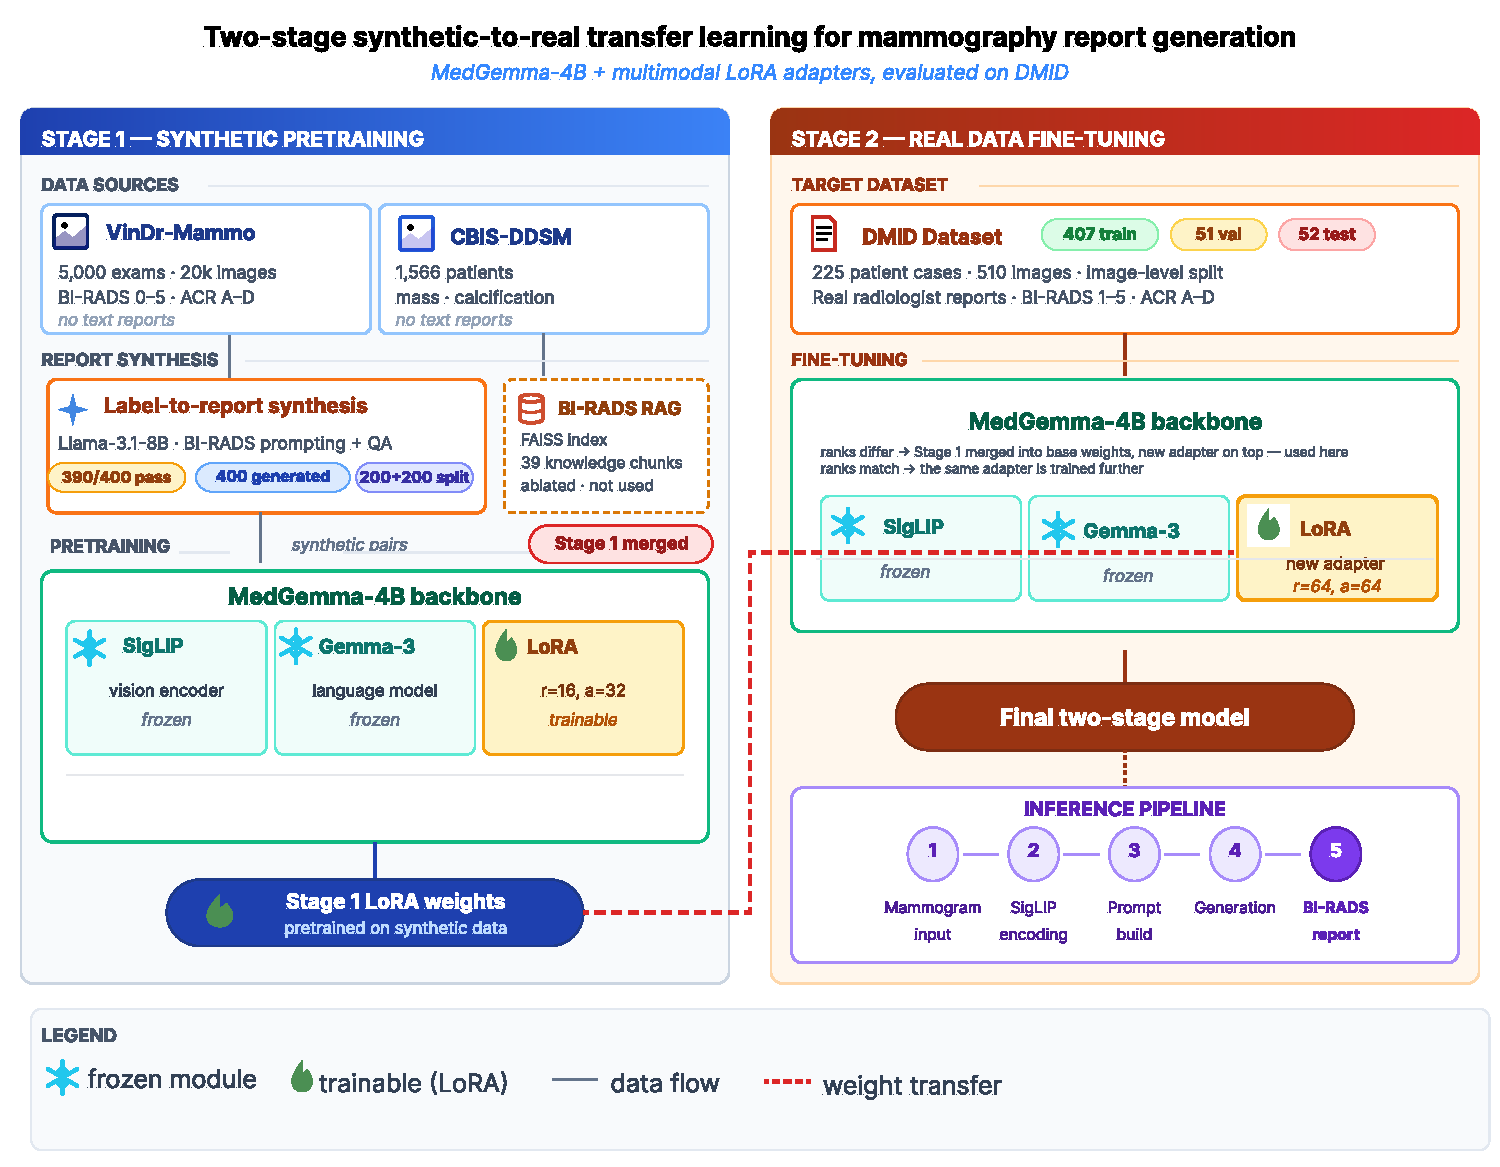
\includegraphics[width=\textwidth]{fig_pipeline_figma.pdf}
\caption{Overview of the two-stage synthetic-to-real transfer learning framework. Stage~1 pretrains on synthetic reports generated from structured BI-RADS annotations in VinDr-Mammo and CBIS-DDSM\revf{: 400 reports are generated and 390 pass automated validation (97.5\%)}. Stage~2 transfers the pretrained LoRA weights and fine-tunes on real radiologist reports from DMID\revf{, by one of two mechanisms---continued training of the same adapter when ranks match, or merging Stage~1 into the base weights (Eq.~\ref{eq:merge}) and training a new adapter otherwise}. \revf{The BI-RADS RAG module is not part of the inference path of the reported models: the retrieval ablation shows that it degrades generation, and it is reported as a negative result. The figure has been redrawn for this revision; the version in the original submission named the wrong report-synthesis model, stated ``100\% QA pass'' instead of 390/400, included a retrieval step in the inference path, and showed a single Stage~1 to Stage~2 transfer arrow where two distinct mechanisms exist.}}
\label{fig:pipeline}
\end{figure}

\subsection*{Datasets}

We use three publicly available mammography datasets (Table~\ref{tab:datasets}).

\begin{table}[H]
\centering
\caption{Dataset characteristics. Only DMID contains paired free-text radiology reports.}
\label{tab:datasets}
\begin{tabular}{lccccc}
\toprule
\textbf{Dataset} & \textbf{Cases} & \textbf{Images} & \textbf{BI-RADS} & \textbf{Density} & \textbf{Reports} \\
\midrule
VinDr-Mammo~\cite{nguyen2023vindr} & 5,000 & 20,000 & 0--5 & A--D & \textcolor{red}{No} \\
CBIS-DDSM~\cite{lee2017curated}      & 1,566 & ---    & 0--5 & ---  & \textcolor{red}{No} \\
DMID~\cite{oza2024}            & 225   & 510    & 1--5 & A--D & \textcolor{hallucinated}{\textbf{Yes}} \\
\bottomrule
\end{tabular}
\end{table}

\textbf{VinDr-Mammo}~\cite{nguyen2023vindr} contains 5,000 four-view screening examinations with breast-level BI-RADS categories, ACR density categories, and finding-level annotations with bounding boxes. \textbf{CBIS-DDSM}~\cite{lee2017curated} contains 1,566 patients with mass and calcification annotations. The INbreast dataset~\cite{moreira2012inbreast}, used in our prior multi-task work~\cite{esen2025multitask}, provides additional mammographic data but also lacks free-text reports. Neither VinDr-Mammo nor CBIS-DDSM contains free-text reports; both are used for Stage~1. \textbf{DMID}~\cite{oza2024} contains 225 cases with paired reports. Following AMRG~\cite{sung2025}, we split DMID into 407 training, 51 validation, and 52 test image-report pairs.

\rev{\textbf{Split granularity and leakage.} The split is \emph{image-level}, not patient-level: DMID distributes 510 images over 225 cases, and the image-to-patient mapping is not published, so a patient-level split cannot be reconstructed from the released files (grouping images by identical report text recovers only 59 complete blocks out of 127). We retain the image-level protocol for comparability with AMRG~\cite{sung2025}, and quantify its consequences rather than leaving them implicit. Grouping the 510 reports by normalised text shows that 3 of the 52 test images (Img462, Img464, Img506) have a report that appears verbatim in the training split. All results below are reported on the full test set ($n=52$); a sensitivity analysis on the 49 remaining cases is given alongside, and changes every metric by 0.014--0.015 ROUGE-L without altering any comparison. A per-image split assignment for all 510 images is provided in Supplementary Table~S1.}

\subsection*{Label-to-Report Synthesis Pipeline}

Given a mammographic image $\mathbf{x}_i$ with structured annotations $\mathbf{a}_i = (l_i, v_i, d_i, f_i, b_i, c_i)$ representing laterality, view position, ACR density, finding categories, BI-RADS assessment, and bounding box coordinates, we construct a structured prompt $\mathbf{p}_i = \phi(\mathbf{a}_i)$ and generate the synthetic report $\hat{r}_i = \mathcal{G}(\mathbf{p}_i)$ using Llama-3.1-8B~\cite{dubey2024llama3} via local inference (Ollama). Each report undergoes quality validation:
\begin{equation}
\mathcal{V}(\hat{r}_i) = \mathbb{1}[\text{BIRADS}(\hat{r}_i)] \cdot \mathbb{1}[\text{Rec}(\hat{r}_i)] \cdot \mathbb{1}[|\hat{r}_i| \geq \tau]
\label{eq:validation}
\end{equation}
where $\mathbb{1}[\cdot]$ denotes indicator functions for BI-RADS mention, recommendation presence, and minimum length $\tau=25$ words\del{, and semantic consistency}. \rev{We note that the version of Eq.~(\ref{eq:validation}) printed in the original submission additionally contained a semantic-consistency term $\mathbb{1}[\text{Sem}(\hat{r}_i, \mathbf{a}_i)]$; no such check was implemented in the released code, and the equation above states the three indicators that were actually applied. A semantic-consistency check comparing the BI-RADS category and laterality asserted in $\hat{r}_i$ against $\mathbf{a}_i$ was added during revision and is reported separately below.}

\rev{Of $400$ generated reports, $390$ satisfied $\mathcal{V}(\hat{r}_i)=1$ and were retained ($196/200$ from VinDr-Mammo, $194/200$ from CBIS-DDSM), yielding $\mathcal{D}_{\text{syn}} = \{(\mathbf{x}_i, \hat{r}_i)\}_{i=1}^{390}$. The validation is fully automated and lexical: it verifies that the three indicators above are present, and does not assess clinical correctness. We therefore avoid the term \emph{clinically validated} for this corpus.}\delpar{original text stated that all 400 reports were retained and described the corpus as clinically validated}

\rev{\textbf{Language contamination.} A post-hoc audit of the retained corpus found that $21$ of the $200$ VinDr-Mammo reports were generated in Russian despite an English-only prompt, and passed validation because the BI-RADS and recommendation indicators are matched case-insensitively on numerals and on terms that survive transliteration. These $21$ reports constitute $5.4\%$ of the $390$-report Stage~1 corpus. They were present in the Stage~1 data used for all experiments reported here; their effect is quantified by the corpus-size sweep in the equivalence analysis below, which uses a rebuilt corpus containing no Cyrillic text.}

\subsection*{BI-RADS Knowledge Base and RAG Module}

The knowledge base $\mathcal{K} = \{k_1, \ldots, k_M\}$ consists of $M=39$ text passages from the ACR BI-RADS Atlas~\cite{birads2013}. Our RAG module~\cite{lewis2020rag} encodes each passage using a sentence transformer~\cite{reimers2019sentencebert} $E_{\text{sent}}$:
\begin{equation}
\mathbf{e}_j = E_{\text{sent}}(k_j) \in \mathbb{R}^{d}, \quad j = 1, \ldots, M
\end{equation}
and indexed in a FAISS~\cite{johnson2020faiss} flat inner product index. At inference, the retrieved context is:
\begin{equation}
k^* = \underset{k_j \in \mathcal{K}}{\arg\max} \; \frac{\mathbf{e}_q^\top \mathbf{e}_j}{\|\mathbf{e}_q\| \|\mathbf{e}_j\|}
\end{equation}

\subsection*{Model Architecture and LoRA Formulation}

We select MedGemma-4B~\cite{lin2024medgemma} comprising a SigLIP~\cite{zoph2020siglip} vision encoder and Gemma-3 language backbone. For a pretrained weight matrix $\mathbf{W}_0 \in \mathbb{R}^{d \times k}$, LoRA~\cite{hu2022lora} constrains the update to a low-rank decomposition:
\begin{equation}
\mathbf{W} = \mathbf{W}_0 + \frac{\alpha}{r}\mathbf{B}\mathbf{A}
\label{eq:lora}
\end{equation}
where $\mathbf{A} \in \mathbb{R}^{r \times k}$, $\mathbf{B} \in \mathbb{R}^{d \times r}$, $r \ll \min(d,k)$, and $\alpha$ is the scaling factor. We apply LoRA to seven target modules per transformer block ($\mathbf{W}_q, \mathbf{W}_k, \mathbf{W}_v, \mathbf{W}_o, \mathbf{W}_{\text{gate}}, \mathbf{W}_{\text{up}}, \mathbf{W}_{\text{down}}$) with default $r=16$, $\alpha=32$, dropout $0.05$:
\begin{equation}
|\Theta_{\text{LoRA}}| = L \cdot n_{\text{modules}} \cdot r \cdot (d + k) \approx 32.8\text{M} \;(0.76\%)
\end{equation}
The base model is quantised to 4-bit using NF4 quantisation following QLoRA~\cite{dettmers2024qlora, dettmers2022gptint8}, enabling training on a single GPU with 32~GB VRAM.

\subsection*{Training Objective}

Both stages optimise the autoregressive language modelling objective. Given vision tokens $\mathbf{z} = E_{\text{vis}}(\mathbf{x})$ and text tokens $\mathbf{t} = (t_1, \ldots, t_T)$:
\begin{equation}
\mathcal{L} = -\sum_{i=1}^{T} \log P_\theta(t_i \mid \mathbf{z}, t_1, \ldots, t_{i-1})
\label{eq:loss}
\end{equation}
where only report tokens contribute (prompt tokens are masked with label $-100$).

\subsection*{Two-Stage Training}

Our approach aligns with established transfer learning principles~\cite{pan2010transfer, zhuang2021survey}, where synthetic pretraining provides domain-adapted initialisation. In Stage~1, LoRA parameters are optimised on synthetic data:
\begin{equation}
\Theta^{(1)} = \underset{\Theta}{\arg\min} \; \frac{1}{|\mathcal{D}_{\text{syn}}|} \sum_{(\mathbf{x}, \hat{r}) \in \mathcal{D}_{\text{syn}}} \mathcal{L}(\mathbf{x}, \hat{r}; \Theta)
\end{equation}
In Stage~2, pretrained parameters $\Theta^{(1)}$ initialise further optimisation on real DMID data:
\begin{equation}
\Theta^{(2)} = \underset{\Theta}{\arg\min} \; \frac{1}{|\mathcal{D}_{\text{real}}|} \sum_{(\mathbf{x}, r) \in \mathcal{D}_{\text{real}}} \mathcal{L}(\mathbf{x}, r; \Theta), \quad \Theta \leftarrow \Theta^{(1)}
\label{eq:stage2}
\end{equation}

\rev{\textbf{Two transfer mechanisms.} Equation~(\ref{eq:stage2}) describes continued training of the \emph{same} adapter, which requires the Stage~1 and Stage~2 adapters to share rank and scaling. When Stage~2 uses a different rank, this is impossible, and Stage~1 is instead merged into the base weights}
\begin{equation}
\revm{\mathbf{W}_0' = \mathbf{W}_0 + \frac{\alpha_1}{r_1}\mathbf{B}_1\mathbf{A}_1 ,}
\label{eq:merge}
\end{equation}
\rev{after which a freshly initialised adapter $\mathbf{B}_2\mathbf{A}_2$ of arbitrary rank $r_2$ is trained on top of $\mathbf{W}_0'$. Both mechanisms were used in the original submission---continuation for the $r=16$ configuration, merging for all others---and the two are not interchangeable: they differ in how much of Stage~1 remains trainable. Because this difference was confounded with adapter rank in the original ablation, every configuration reported here was retrained under the merging mechanism of Eq.~(\ref{eq:merge}), so that all rows of Table~\ref{tab:lora} differ only in $r$ and $\alpha$.}

\subsection*{Implementation Details}

Stage~1: 3 epochs, AdamW, lr $2 \times 10^{-4}$, cosine schedule, warm-up 100 steps, batch 8, images $448 \times 448$, 4-bit NF4 quantisation. Stage~2: 5 epochs, lr $1 \times 10^{-4}$, warm-up 20 steps, batch 1 $\times$ gradient accumulation 8, best model at epoch 4 (val loss 0.655). All training on a single NVIDIA RTX 5090 (32 GB VRAM). Stage~1 training time: $\sim$3 minutes; Stage~2: $\sim$37 minutes.

\rev{\textbf{Unified evaluation protocol.} All models reported in this revision were re-evaluated under one protocol: 4-bit NF4 quantisation, $448\times448$ input, greedy decoding, 200 new tokens, a single instruction prompt used at both training and evaluation time, and a single rule for extracting the BI-RADS category and ACR density from generated text. Per-sample generations are stored for every model, so that confidence intervals, paired tests and clinical metrics are recomputable without re-running inference.}

\rev{\textbf{Prompt mismatch in the original evaluation.} Two instruction prompts were used in the original work. The $r=16$ models were trained with the prompt \emph{``Generate a structured mammography report with breast composition, findings, BI-RADS category and recommendation''}, whereas evaluation was carried out with the variant used for the ablation configurations, \emph{``Generate a structured mammography radiology report with breast composition (ACR density), findings, BI-RADS category, and recommendation''}. The mismatch penalises the two models unequally: re-evaluating each $r=16$ model under its own training prompt raises ROUGE-L by $0.0140$ for DMID-only but only by $0.0033$ for two-stage. The gap between the two branches at $r=16$ therefore shrinks from $0.0579$ to $0.0472$, so about one fifth of it is an artefact of the evaluation prompt rather than of synthetic pretraining. All numbers in this revision use matched training and evaluation prompts.}

\subsection*{Evaluation Protocol}

\textbf{Automated NLP metrics}: BLEU-1/4~\cite{papineni2002bleu}, ROUGE-1/2/L~\cite{lin2004rouge}, METEOR~\cite{banerjee2005meteor}, CIDEr~\cite{vedantam2015cider}, and BERTScore~\cite{zhang2020bertscore}. CIDEr is computed using pycocoevalcap. \textbf{Clinical metrics}: BI-RADS accuracy, recommendation accuracy, \rev{finding-level sensitivity, omission rate and hallucination rate}.

\rev{\textbf{Definition of hallucination and omission.} The original submission scored a report as hallucinated when a clinical term occurred in the generated text but not verbatim in the reference. That criterion measures lexical divergence, not invention: a report stating \emph{``no abnormal soft opacity''} is counted as hallucinating \emph{opacity}. We replace it with an assertion-level definition. A finding is \emph{asserted} in a report if a finding term occurs without a negation cue within a 45-character window. Writing $A(\cdot)$ for the set of findings asserted in a text, for reference $r$ and generation $\hat{r}$:}
\begin{equation}
\revm{\text{hallucination} = \frac{|A(\hat{r}) \setminus A(r)|}{|A(\hat{r})|}, \qquad
      \text{omission} = \frac{|A(r) \setminus A(\hat{r})|}{|A(r)|}, \qquad
      \text{sensitivity} = 1 - \text{omission} .}
\label{eq:halluc}
\end{equation}
\rev{Under this definition the failure mode of every fine-tuned model in this study is omission, not invention (Table~\ref{tab:clinical}), which reverses the clinical reading of the original hallucination numbers.}

\textbf{Baselines}: We compare against LLaVA-1.6~\cite{liu2024llava}, Qwen2.5-VL~\cite{wang2024qwen2vl}, and pipeline approaches using CLIP~\cite{radford2021clip} with GPT-2~\cite{radford2019gpt2}. \rev{A tenth model, Phi-3.5-vision, was run but produced no parseable report on any test image; all of its metrics are identically zero and it is excluded from the tables rather than reported as a score of zero. The comparison therefore spans eight methods besides our own.}

\rev{\textbf{Statistical analysis.} The original submission compared the two branches with a permutation test that shuffled the two score vectors as independent samples. Because both models are evaluated on the same 52 images, the samples are paired and the test was mis-specified. We use a paired permutation test on the per-image differences $d_i = m(\hat{r}_i^{A}) - m(\hat{r}_i^{B})$, randomising the sign of each difference over $N_{\text{perm}} = 10{,}000$ draws $\mathbf{s} \in \{-1,+1\}^{n}$:}
\begin{equation}
\revm{p = \frac{1}{N_{\text{perm}}} \sum_{j=1}^{N_{\text{perm}}} \mathbb{1}\!\left[\,\bigl|\overline{\mathbf{s}_j \odot \mathbf{d}}\bigr| \geq \bigl|\bar{d}\bigr|\,\right]}
\end{equation}
\rev{and report bias-corrected and accelerated (BCa) bootstrap confidence intervals with 10{,}000 resamples for every metric of every model. BLEU and CIDEr are corpus-level statistics by definition; where they appear in paired comparisons they are computed per sample, and the two conventions are not mixed within a table.}

\rev{\subsection*{Evaluation by radiologists}

We did not carry out a reader study for this revision. An offline evaluation instrument was built for the purpose---an image-first, two-stage protocol in which the radiologist records what the image shows before the generated report is revealed, then rates the report on five ordinal axes and marks any clinically significant finding omitted from it---and it is released together with the code so that the study can be run and audited by others. Securing the required hours from board-certified radiologists was not possible within the revision period, and we prefer to state this plainly rather than substitute a weaker form of expert assessment. The absence of radiologist evaluation is recorded in Limitations, and no claim in this paper rests on expert reading: the clinical figures we report are computed from the reference DMID reports under the explicit definitions given above.}

%% ─────────────────────────────────────────────────────────────────
\section*{Results}
%% ─────────────────────────────────────────────────────────────────

\subsection*{Stage~1: Synthetic Data Evaluation}

Table~\ref{tab:synthetic} presents Stage~1 evaluation on held-out synthetic data ($n=30$). Our multimodal fine-tuned model achieves ROUGE-1 of 0.612 and BERTScore of 0.919, significantly outperforming all zero-shot baselines ($p < 0.0001$).

\begin{table}[H]
\centering
\caption{Stage~1 evaluation on synthetic test data ($n=30$). Best values in bold.}
\label{tab:synthetic}
\begin{tabular}{lcccccc}
\toprule
\textbf{Method} & \textbf{BLEU-1} & \textbf{BLEU-4} & \textbf{ROUGE-1} & \textbf{ROUGE-L} & \textbf{BERTScore} \\
\midrule
LLaVA-1.6-7B (zero-shot)        & 0.074 & 0.001 & 0.221 & 0.136 & 0.818 \\
MedGemma-4B (zero-shot)          & 0.201 & 0.037 & 0.365 & 0.236 & 0.843 \\
Qwen2.5-VL-7B (zero-shot)       & 0.241 & 0.054 & 0.412 & 0.250 & 0.860 \\
Text FT + RAG                    & 0.331 & 0.101 & 0.456 & 0.336 & 0.880 \\
Multimodal FT + RAG              & 0.246 & 0.069 & 0.423 & 0.270 & 0.876 \\
\textbf{Multimodal FT (Stage~1)} & \textbf{0.444} & \textbf{0.182} & \textbf{0.612} & \textbf{0.480} & \textbf{0.919} \\
\bottomrule
\end{tabular}
\end{table}
\subsection*{Stage~2: DMID Real-Data Evaluation}

Table~\ref{tab:dmid} presents the primary evaluation on the DMID test set ($n=52$) against real radiologist reports across \rev{eight baseline} methods spanning four architectural paradigms: zero-shot VLMs, pipeline models (CLIP/MedCLIP + GPT2), direct fine-tuning\rev{, and the previously reported state of the art}\rev{. Both training schemes are shown at two adapter ranks, so that each comparison between them is made at matched capacity}.

\begin{table}[H]
\centering
\caption{DMID test set evaluation against real radiologist reports ($n=52$). \revf{The two training schemes are shown at matched adapter rank: the original submission compared DMID-only at $r=16$ with two-stage at $r=64$, so that the reported gap confounded training scheme with adapter capacity. Best value per column in bold. BERTScore is recomputed for all rows we trained under a single protocol (roberta-large, no baseline rescaling); the value of 0.917 given in the original submission for the two-stage row originated from a different run. CIDEr for the pipeline baselines, previously left empty, is now reported. Neither final model uses retrieval at inference (see the RAG ablation below). AMRG numbers are quoted from~\cite{sung2025} and were obtained on a different split with a different category-extraction rule, so that row is not directly comparable; its BLEU-4 entry is withdrawn because the source reports BLEU-1 only.}}
\label{tab:dmid}
\begin{adjustbox}{max width=\textwidth}
\begin{tabular}{llccccccc}
\toprule
\textbf{Method} & \textbf{Type} & \textbf{BLEU-1} & \textbf{BLEU-4} & \textbf{ROUGE-1} & \textbf{ROUGE-L} & \textbf{METEOR} & \textbf{CIDEr} & \textbf{BERTSc.} \\
\midrule
LLaVA-1.6-7B         & VLM, ZS    & 0.059 & 0.001 & 0.157 & 0.109 & 0.188 & 0.005 & 0.810 \\
MedGemma-4B           & VLM, ZS    & 0.061 & 0.001 & 0.151 & 0.098 & 0.192 & 0.000 & \revf{0.805} \\
Qwen2.5-VL-7B        & VLM, ZS    & 0.072 & 0.002 & 0.202 & 0.145 & 0.207 & 0.009 & 0.823 \\
Qwen3-VL-8B          & VLM, ZS    & 0.108 & 0.002 & 0.236 & 0.147 & 0.228 & 0.007 & ---   \\
MedCLIP+GPT2          & Pipeline, FT & 0.378 & 0.217 & 0.648 & 0.571 & 0.555 & \revf{0.054}   & 0.905 \\
CLIP+GPT2             & Pipeline, FT & 0.384 & 0.238 & 0.673 & 0.613 & 0.591 & \revf{0.078}   & 0.909 \\
AMRG~\cite{sung2025} & VLM, FT    & 0.308 & \revf{---} & 0.575 & 0.569 & 0.615 & 0.582 & ---   \\
\midrule
DMID-only, $r{=}16$      & VLM, FT    & 0.442 & 0.203 & 0.676 & 0.601 & 0.597 & 0.455 & \revf{0.908} \\
\revf{Two-stage, $r{=}16$} & \revf{VLM, 2S-FT} & \revf{0.498} & \revf{0.278} & \revf{0.719} & \revf{0.659} & \revf{0.657} & \revf{0.639} & \revf{0.916} \\
\revf{DMID-only, $r{=}64$} & \revf{VLM, FT} & \revf{\textbf{0.542}} & \revf{\textbf{0.315}} & \revf{\textbf{0.738}} & \revf{0.670} & \revf{\textbf{0.691}} & \revf{0.693} & \revf{\textbf{0.920}} \\
\revf{Two-stage, $r{=}64$} & \revf{VLM, 2S-FT} & \revf{0.530} & \revf{0.312} & \revf{0.734} & \revf{\textbf{0.671}} & \revf{0.685} & \revf{\textbf{0.729}} & \revf{0.919} \\
\bottomrule
\end{tabular}
\end{adjustbox}
\end{table}

\rev{At matched capacity the two training schemes are not distinguishable. At $r=64$ the DMID-only baseline attains the best value in five of the seven columns, and two-stage leads only on ROUGE-L (by $0.0009$) and CIDEr; the ordering of the two branches therefore depends on which metric is chosen. The apparent advantage of the two-stage model in the original submission was measured between models of different capacity: comparing DMID-only at $r=16$ (ROUGE-L $0.601$) with two-stage at $r=64$ ($0.671$) mixes a capacity effect with a training-scheme effect. Increasing adapter rank from $16$ to $64$ raises the DMID-only baseline from $0.601$ to $0.670$, which accounts for essentially the whole of the originally reported difference.}

\rev{Table~\ref{tab:equalcap} gives the paired comparison at each rank. At $r=64$ no metric separates the branches: all six differences lie within $\pm 0.006$, every confidence interval contains zero, and the smallest $p$-value is $0.48$. At $r=16$ all six metrics favour two-stage with $p=0.0001$. This within-run significance does not survive replication: repeating the $r=16$ comparison over three random initialisations shrinks the ROUGE-L difference to $+0.003$, against a between-run standard deviation of $0.039$--$0.045$ at this rank (see the equivalence analysis below). We report both facts together because they carry a methodological consequence beyond this study: at this sample size a correctly specified paired test can return $p=0.0001$ for an effect that does not reproduce across initialisations. A confidence interval over cases and a confidence interval over initialisations answer different questions, and a claim of method superiority requires the second.}

\begin{table}[H]
\centering
\caption{\revf{Paired comparison of the two training schemes at matched adapter rank on the DMID test set ($n=52$). $\Delta$ is two-stage minus DMID-only, computed per image; intervals are 95\% BCa bootstrap intervals with 10{,}000 resamples; $p$ is a paired permutation test with sign randomisation over 10{,}000 draws. The $r=16$ column reproduces the published comparison under matched prompts; the $r=64$ column is the comparison at equal capacity.}}
\label{tab:equalcap}
\begin{adjustbox}{max width=\textwidth}
\begin{tabular}{lcccccc}
\toprule
& \multicolumn{3}{c}{$r=16$} & \multicolumn{3}{c}{$r=64$} \\
\cmidrule(lr){2-4} \cmidrule(lr){5-7}
\textbf{Metric} & $\Delta$ & \textbf{95\% CI} & $p$ & $\Delta$ & \textbf{95\% CI} & $p$ \\
\midrule
BLEU-1  & $+0.0676$ & $[+0.0429, +0.0888]$ & $0.0001$ & $-0.0040$ & $[-0.0255, +0.0103]$ & $0.68$ \\
BLEU-4  & $+0.0805$ & $[+0.0604, +0.1016]$ & $0.0001$ & $+0.0011$ & $[-0.0086, +0.0098]$ & $0.83$ \\
ROUGE-1 & $+0.0439$ & $[+0.0266, +0.0586]$ & $0.0001$ & $-0.0044$ & $[-0.0234, +0.0066]$ & $0.56$ \\
ROUGE-2 & $+0.0876$ & $[+0.0644, +0.1136]$ & $0.0001$ & $-0.0005$ & $[-0.0223, +0.0118]$ & $0.95$ \\
ROUGE-L & $+0.0579$ & $[+0.0393, +0.0755]$ & $0.0001$ & $+0.0009$ & $[-0.0171, +0.0154]$ & $0.92$ \\
METEOR  & $+0.0603$ & $[+0.0329, +0.0852]$ & $0.0001$ & $-0.0061$ & $[-0.0291, +0.0046]$ & $0.48$ \\
\bottomrule
\end{tabular}
\end{adjustbox}
\end{table}

\rev{Excluding the three test images whose reference report appears verbatim in the training split leaves every conclusion unchanged: all metrics fall by $0.014$--$0.015$ ROUGE-L for all models, and the difference at $r=64$ becomes $+0.0010$ with 95\% CI $[-0.0186, +0.0162]$, $p=0.92$.}

\delpar{Our two-stage model achieves the highest scores across all reported metrics. Compared to AMRG, our approach yields improvements of +17.9\% in ROUGE-L, +11.4\% in METEOR and +25.3\% in CIDEr. The improvement over the DMID-only baseline is statistically significant (p=0.045, bootstrap permutation test on ROUGE-L).}

\rev{Against AMRG~\cite{sung2025}, all four of our fine-tuned configurations score higher on every text metric. We report this comparison with an explicit caveat: AMRG's numbers were obtained on a different split of DMID and with a different rule for extracting BI-RADS categories, and we did not re-run their system under our protocol. The comparison establishes that our models are competitive with published work, not that a specific component of our framework is responsible for the difference.}
\begin{figure}[H]
\centering
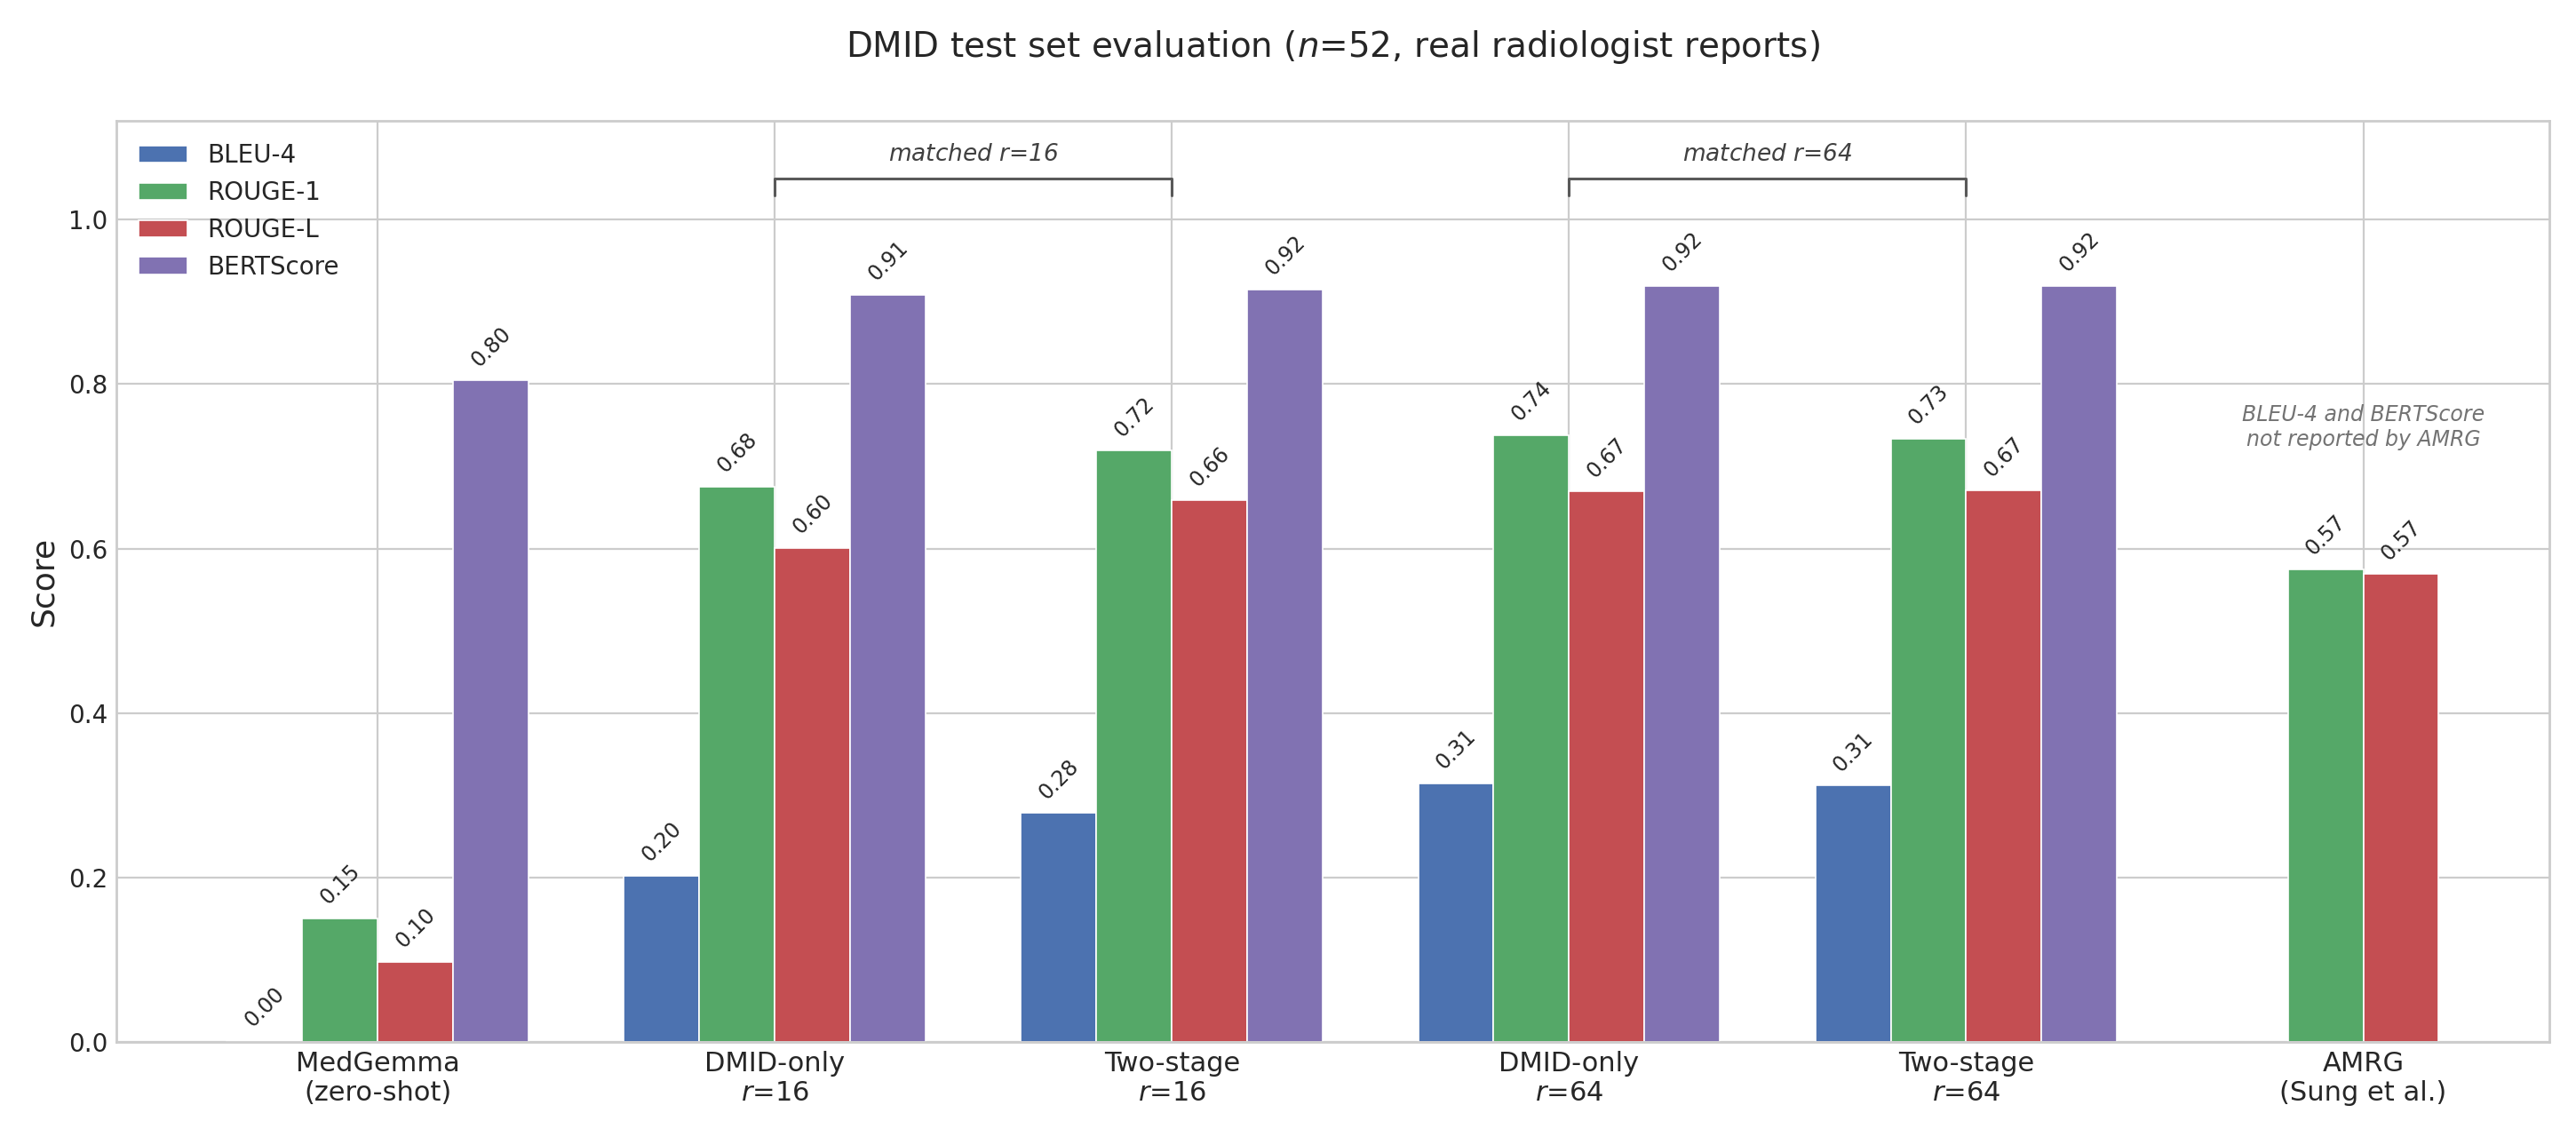
\includegraphics[width=\textwidth]{fig_dmid_ablation.png}
\caption{DMID test set comparison across key methods ($n=52$)\revf{, with the two training schemes shown at matched adapter rank. The figure has been regenerated: the version in the original submission plotted DMID-only at $r=16$ against two-stage at $r=64$ and so repeated the capacity confound corrected in Table~\ref{tab:dmid}. At $r=64$ the two schemes are visually indistinguishable on every metric}.}
\label{fig:dmid_bar}
\end{figure}
\subsection*{Clinical Metric Evaluation}

Table~\ref{tab:clinical} presents clinical quality metrics. In this evaluation, the model must predict clinical attributes directly from mammographic images without any BI-RADS input.

\begin{table}[H]
\centering
\caption{\revf{Clinical quality metrics on the DMID test set ($n=52$), all models at matched adapter rank. Hallucination and omission follow the assertion-level definition of Eq.~(\ref{eq:halluc}); density accuracy is computed on all 52 cases rather than on a hand-picked subset. ``Downgraded'' counts reference-suspicious cases (BI-RADS 4--5, $n=22$) that the model assigned to BI-RADS 1--2, the clinically most consequential error.}}
\label{tab:clinical}
\begin{adjustbox}{max width=\textwidth}
\begin{tabular}{lcccccccc}
\toprule
& \multicolumn{3}{c}{\textbf{BI-RADS}} & \multicolumn{3}{c}{\textbf{Findings}} & \multicolumn{2}{c}{\textbf{ACR density}} \\
\cmidrule(lr){2-4} \cmidrule(lr){5-7} \cmidrule(lr){8-9}
\textbf{Method} & \textbf{Exact} & $\kappa$ & \textbf{Downgr.} & \textbf{Sens.} & \textbf{Omis.} & \textbf{Halluc.} & \textbf{Acc.} & $\kappa$ \\
\midrule
MedGemma-4B (ZS)      & \revf{0.333$^\dagger$} & \revf{0.000} & \revf{0/3$^\dagger$}  & \revf{0.300} & \revf{0.700} & \revf{0.000} & \revf{0.167$^\ddagger$} & \revf{$-0.027$} \\
\midrule
DMID-only, $r{=}16$   & \revf{0.365} & \revf{0.160} & \revf{8/22}  & \revf{\textbf{0.575}} & \revf{0.425} & \revf{0.000} & \revf{0.385} & \revf{0.000} \\
\revf{Two-stage, $r{=}16$} & \revf{0.327} & \revf{0.113} & \revf{10/22} & \revf{0.525} & \revf{0.475} & \revf{0.000} & \revf{\textbf{0.519}} & \revf{0.146} \\
\revf{DMID-only, $r{=}64$} & \revf{0.365} & \revf{0.167} & \revf{7/22}  & \revf{\textbf{0.675}} & \revf{0.325} & \revf{0.000} & \revf{0.462} & \revf{0.000} \\
\revf{Two-stage, $r{=}64$} & \revf{0.365} & \revf{0.168} & \revf{7/22}  & \revf{0.650} & \revf{0.350} & \revf{0.000} & \revf{0.462} & \revf{0.000} \\
\bottomrule
\end{tabular}
\end{adjustbox}

\revf{\footnotesize $^\dagger$Only 3 of 52 zero-shot outputs contain a parseable BI-RADS category; the rate is computed on those 3 and is not comparable with the fine-tuned rows. $^\ddagger$Computed on the 18 zero-shot outputs stating an ACR category.}
\end{table}

\rev{Three results in this table differ from the original submission.}

\rev{\textbf{The models do not fabricate findings; they omit them.} Under the assertion-level definition of Eq.~(\ref{eq:halluc}) the hallucination rate is $0.000$ for every model, including the zero-shot baseline, while omission ranges from $0.325$ to $0.700$. The reduction from $73.1\%$ to $\sim\!20\%$ reported previously was an artefact of the lexical criterion, which counted a negated mention such as \emph{``no abnormal soft opacity''} as a hallucinated \emph{opacity}; fine-tuning shortens reports and aligns their vocabulary with the references, which lowers that score without any change in fabrication. The clinically relevant statement is the opposite of the original one: the dominant error of these models is silence about findings that are present. Of the 52 reference reports, 40 assert at least one finding; the best model (DMID-only, $r=64$) fails to assert a finding in 13 of those 40 cases, that is $32.5\%$ of the cases with a finding and $25.0\%$ of the test set. We state both denominators explicitly because they are not interchangeable.}

\rev{\textbf{Synthetic pretraining does not improve finding detection.} At both ranks the DMID-only baseline has the higher sensitivity ($0.575$ vs.\ $0.525$ at $r=16$; $0.675$ vs.\ $0.650$ at $r=64$).}

\rev{\textbf{The density result does not survive full evaluation.} The claim that the two-stage model predicts density better rested on 5 hand-picked cases (4/5 vs.\ 1/5). Computed on all 52 cases, both $r=64$ models score $0.462$ with $\kappa = 0$: they assign ACR B to every case, and their accuracy is the prevalence of ACR B in the test set, not evidence of density perception. The same holds for DMID-only at $r=16$. The one configuration with non-trivial density agreement is two-stage at $r=16$ ($\kappa = 0.146$), which is also the configuration with the worst BI-RADS agreement in the table. Occasional per-seed exceptions to $\kappa \approx 0$ occur but do not reproduce across initialisations.}

\rev{Generated reports average $37.1$ words (two-stage, $r=64$) and $38.3$ words (DMID-only, $r=64$) against $43.1$ words for the reference reports, compared with $118.7$ words for the zero-shot baseline; fine-tuning calibrates report length, and the two schemes are indistinguishable in this respect as well.}

\subsection*{BI-RADS Distribution and Per-Category Analysis}

The DMID test set exhibits the following BI-RADS distribution: BI-RADS 1 (21.2\%, $n=11$), BI-RADS 2 (13.5\%, $n=7$), BI-RADS 3 (23.1\%, $n=12$), BI-RADS 4 (28.8\%, $n=15$), and BI-RADS 5 (13.5\%, $n=7$). Breast density distribution spans ACR A (5.8\%), ACR B (46.2\%), ACR C (38.5\%), and ACR D (9.6\%).

\rev{The predominance of ACR B density in the test set (46.2\%) explains the density accuracy of both $r=64$ models without any appeal to density perception. Both assign ACR B to all 52 cases, so their accuracy of $0.462$ is exactly the prevalence of ACR B and their agreement with the reference is $\kappa = 0$. VinDr-Mammo, on which Stage~1 is built, is likewise dominated by ACR B, so the constant prediction is consistent with inheriting the majority class of the pretraining distribution rather than with transferring density knowledge. The corresponding claim in the original submission---that two-stage predicts density better than DMID-only, which defaults to ACR C---was based on 5 hand-picked cases and does not hold on the full test set.}\delpar{original paragraph attributed the ACR B prediction to density knowledge transferred from VinDr-Mammo and the ACR C default of DMID-only to insufficient learning}

\rev{The overall BI-RADS accuracy of $0.365$ masks substantial variation across categories, and the variation runs in the clinically unfavourable direction. Normal cases (BI-RADS 1--2) are identified far more reliably than suspicious ones: of the 22 reference-suspicious cases, 7 are assigned to BI-RADS 1--2 by both $r=64$ models. Agreement beyond chance is low for every model in this study ($\kappa$ between $0.08$ and $0.17$). This is consistent with the clinical difficulty of distinguishing subtle malignant features~\cite{sechopoulos2021artificial}, and it is the principal obstacle to any clinical use of these outputs; class-balanced training or BI-RADS-specific loss weighting remain plausible directions, but the gap is large enough that we do not present the current accuracy as adequate for assistance in reporting.}

\rev{Fine-tuning does change output behaviour substantially, but not in the way the original submission described. In the zero-shot setting MedGemma-4B~\cite{lin2024medgemma} produces verbose, unstructured responses averaging $118.7$ words, only 3 of which contain a parseable BI-RADS category, whereas every fine-tuned model produces a BI-RADS category and an ACR category in all 52 cases and averages $37$--$38$ words against $43.1$ for the references. What fine-tuning delivers is structural conformity and length calibration. It does not reduce fabrication, because under an assertion-level criterion no model fabricates findings at any stage; and it does not improve category agreement beyond $\kappa \approx 0.17$.}\delpar{original paragraph reported a hallucination reduction from 73.1\% to about 20\% and a mean length of 42.2 words}

\subsection*{Data Efficiency Analysis}

Figure~\ref{fig:efficiency} presents the data efficiency analysis across varying amounts of real training data; the underlying numbers are given in Supplementary Table~S2.


\rev{Within this experiment the two-stage curve lies above the DMID-only curve at every data volume. We do not draw a data-efficiency conclusion from it. The differences on which such a conclusion would rest are smaller than the run-to-run variability we measured elsewhere in this study: the gap between two-stage at $N=200$ ($0.599$) and DMID-only at $N=407$ ($0.615$) is $0.0155$, and the margin over the AMRG benchmark at $N=100$ is $0.001$, against a between-initialisation standard deviation of $0.039$--$0.045$ ROUGE-L for a fixed configuration. A single initialisation per point cannot separate these differences from initialisation noise. The claim of a $2\times$ reduction in real-data requirements is therefore withdrawn, and we do not replace it with a weaker quantitative statement.}\delpar{Two key findings emerge. First, synthetic pretraining benefit increases with real data (from +4.0\% to +7.6\%), suggesting complementarity. Second, the two-stage model with 200 real examples approaches the DMID-only model with 407, indicating about 2x data savings. Notably, two-stage with only 100 examples already surpasses the AMRG benchmark.}


\begin{figure}[H]
\centering
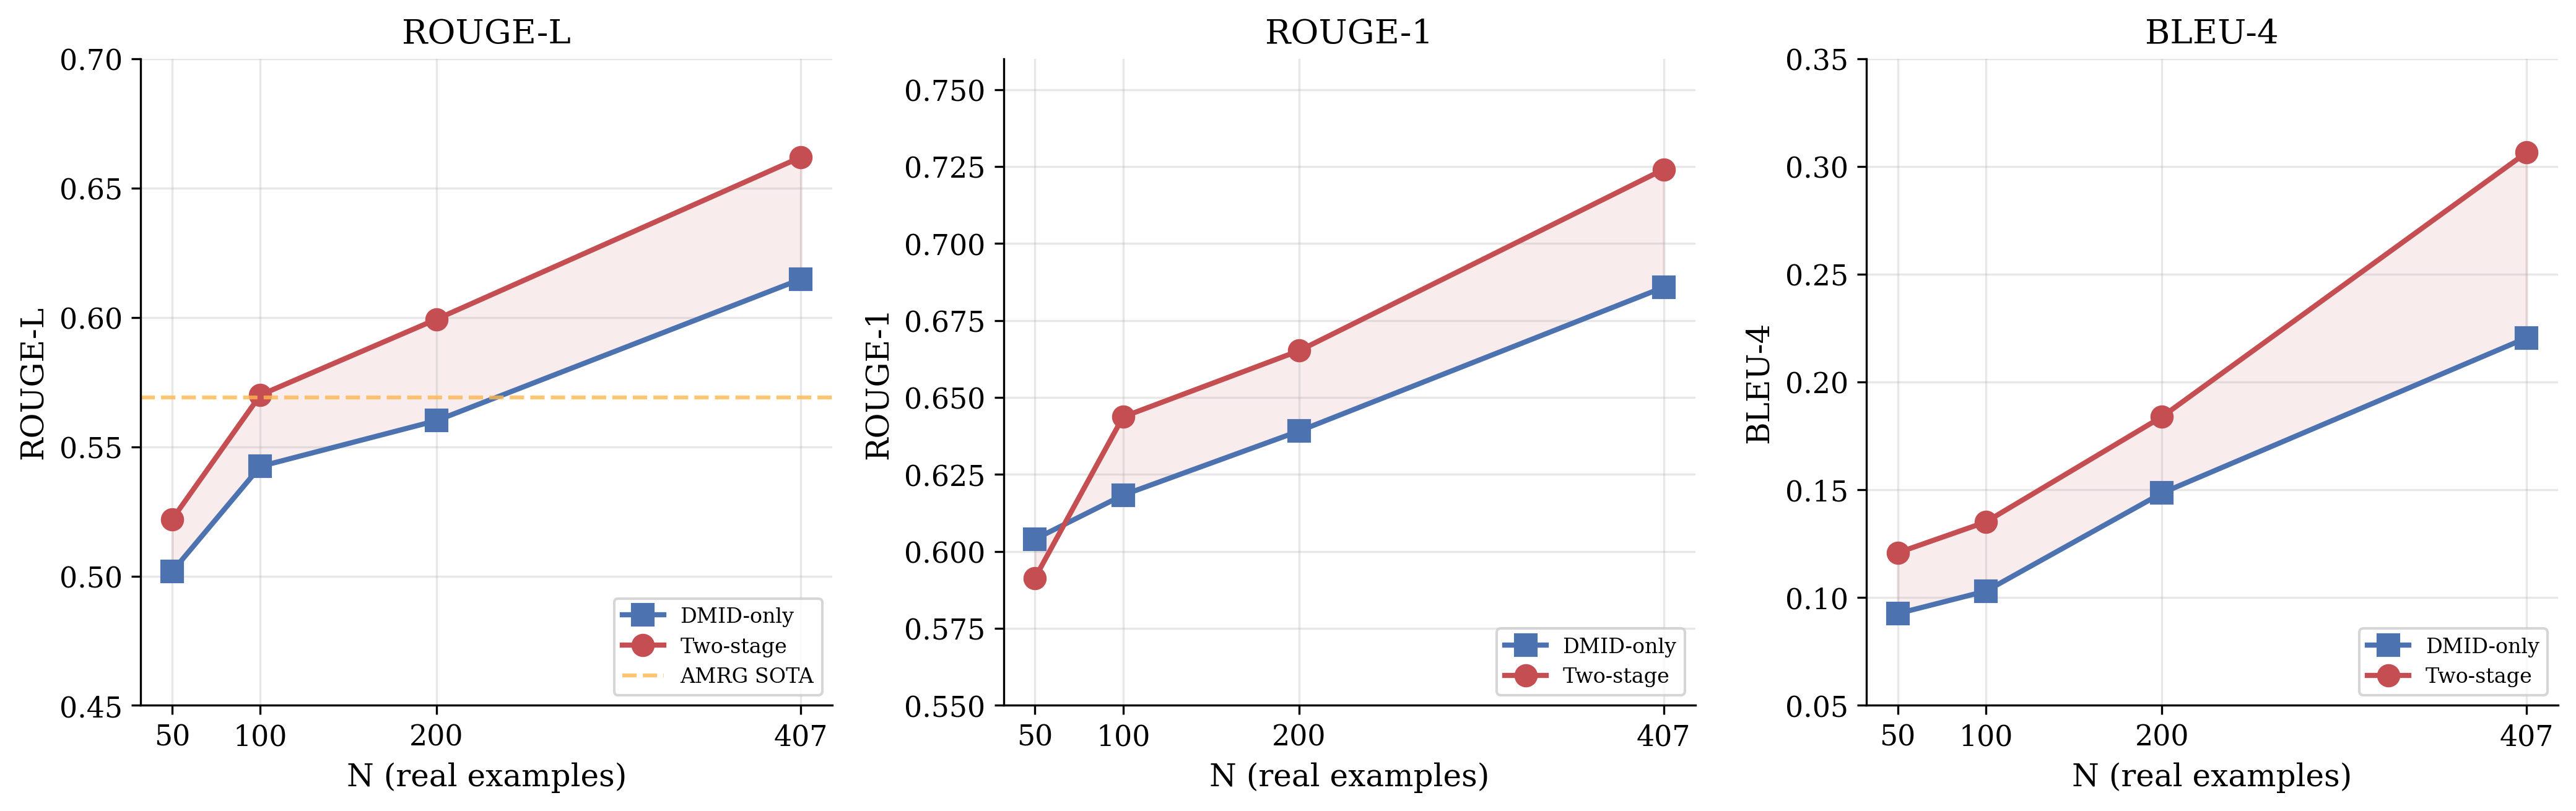
\includegraphics[width=\textwidth]{fig_data_efficiency.png}
\caption{Data efficiency analysis \revf{under the protocol of Supplementary Table~S2 ($r=16$, one initialisation per point). Error bars are unavailable because per-sample generations were not retained; the separation between the curves is smaller than the between-initialisation variability measured for a fixed configuration elsewhere in this study, and no data-efficiency claim is drawn from it}.}\delpar{Synthetic pretraining consistently improves performance and the benefit grows with more real data. Two-stage with N=100 surpasses the AMRG SOTA (dashed line).}
\label{fig:efficiency}
\end{figure}

\subsection*{Training Dynamics}

Figure~\ref{fig:curves} compares training dynamics. The two-stage model starts with lower initial training loss (3.33 vs. 4.00) and achieves lower best validation loss (0.655 vs. 0.669)\rev{, which is consistent with synthetic pretraining providing a domain-adapted initialisation~\cite{pan2010transfer}. The lower starting loss is expected and robust: the Stage~1 adapter has already seen mammography report vocabulary and formatting. The difference in \emph{best} validation loss is a single-run difference of $0.014$ and should not be read as evidence of a better final model, since it does not translate into a difference in test-set output at matched capacity (Table~\ref{tab:equalcap})}\delpar{, confirming that synthetic pretraining provides a more favourable initialisation}.


\begin{figure}[H]
\centering
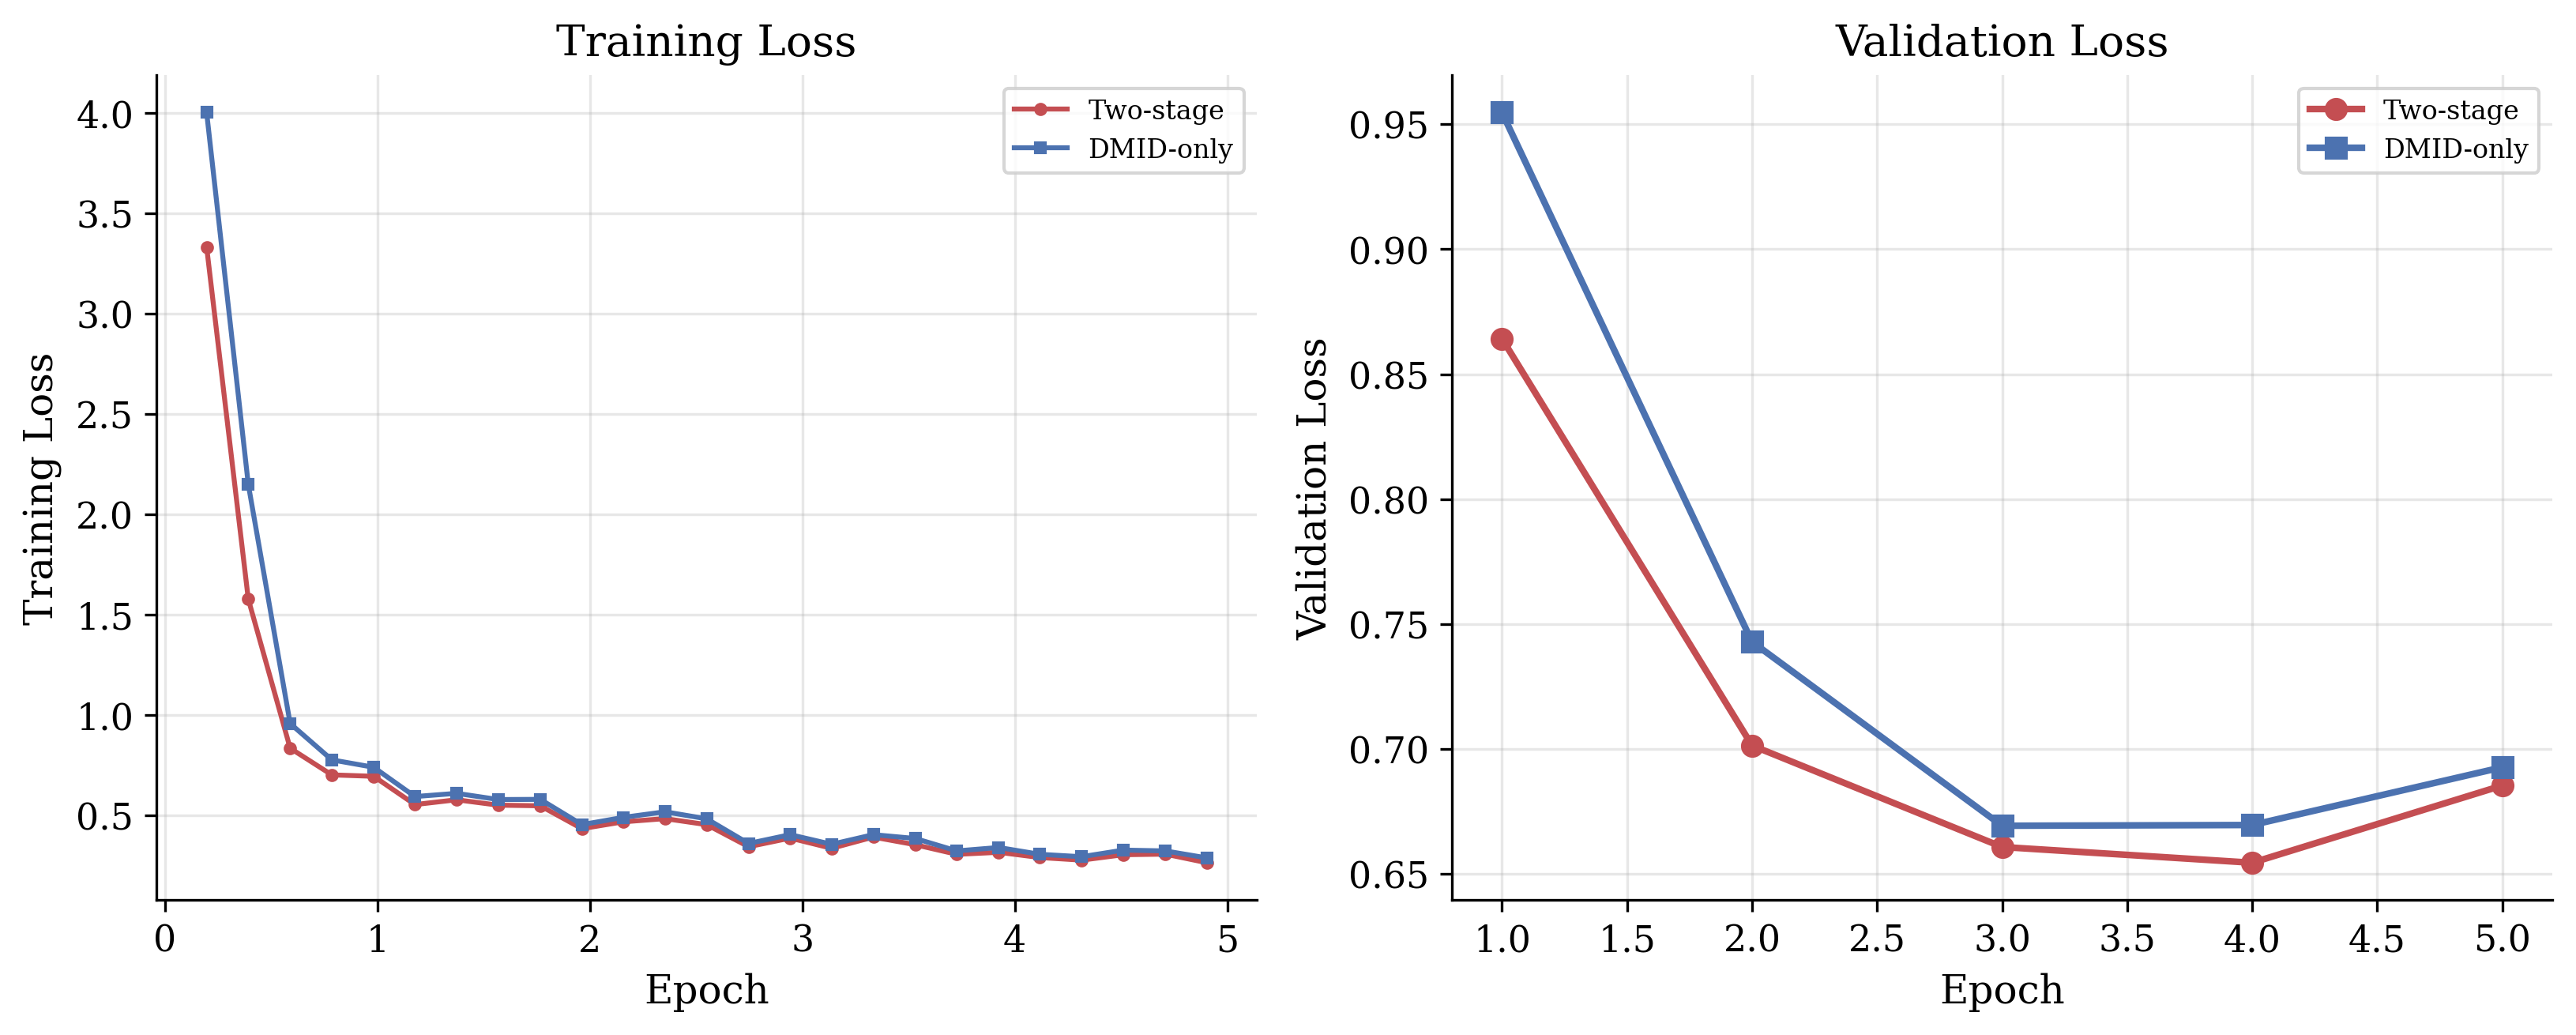
\includegraphics[width=\textwidth]{fig_training_curves.png}
\caption{Training dynamics. Two-stage benefits from lower initial loss and achieves lower best validation loss (0.655 vs. 0.669).}
\label{fig:curves}
\end{figure}

\subsection*{Qualitative Analysis}

\rev{Table~\ref{tab:qualitative} presents representative generated reports with colour-coded clinical term evaluation: \textcolor{correct}{correct terms (blue)}, \textcolor{incorrect}{incorrect terms (red)}, and \textcolor{hallucinated}{findings present in the reference but omitted from the generated report (green)}. The third category was \emph{hallucinated terms} in the original submission; it is redefined here because no fabricated finding occurs in any generation under the criterion of Eq.~(\ref{eq:halluc}), whereas omission is the dominant error. Both branches are shown at $r=64$, the matched-capacity comparison. All three examples are drawn from the 49 test cases whose reference report does not appear in the training split; the example used in the original submission (Img462) is one of the three leaked cases and has been replaced.}

\begin{table}[H]
\centering
\caption{\revf{Qualitative comparison of generated mammography reports at matched adapter rank ($r=64$). Clinical terms: \textcolor{correct}{correct (blue)}, \textcolor{incorrect}{incorrect (red)}, \textcolor{hallucinated}{omitted from the generation (green)}.}}
\label{tab:qualitative}
\small
\begin{tabularx}{\textwidth}{p{1.8cm}p{1.4cm}X}
\toprule
\textbf{Image} & \textbf{Method} & \textbf{Generated Report} \\
\midrule
\multicolumn{3}{l}{\revf{\textbf{Example 1: Img510 --- Normal breast (BI-RADS 1) --- both schemes correct and identical}}} \\
\midrule
\multirow{3}{*}{\includegraphics[width=1.6cm]{mammo_510.png}}
& \textbf{GT} & \revf{BC: \textcolor{correct}{fibro fatty and glandular (ACR B)}. F: \textcolor{correct}{no abnormal soft opacity or microcalcification}. \textcolor{correct}{Skin, nipple and pectoral muscle appear normal}. \textcolor{correct}{No significant axillary nodes}. \textcolor{correct}{BIRADS: 1}} \\
\addlinespace
& \revf{\textbf{Two-stage}} & \revf{BC: \textcolor{correct}{fibro fatty and glandular (ACR B)}. F: \textcolor{correct}{No abnormal soft opacity or microcalcification}. \textcolor{correct}{Skin, nipple and pectoral muscle appear normal}. \textcolor{correct}{No significant axillary adenopathy}. \textcolor{correct}{BIRADS: 1}} \\
\addlinespace
& \revf{\textbf{DMID-only}} & \revf{\emph{token-identical to the two-stage output above}} \\
\midrule
\multicolumn{3}{l}{\revf{\textbf{Example 2: Img501 --- Malignant lesion (BI-RADS 5) --- both schemes fail identically}}} \\
\midrule
\multirow{3}{*}{\includegraphics[width=1.6cm]{mammo_501.png}}
& \textbf{GT} & \revf{BC: \textcolor{correct}{dense glandular (ACR D)}. F: \textcolor{hallucinated}{a large well defined lobulated soft opacity with foci of microcalcifications in the posterior aspect of the outer quadrant, suggesting malignant lesion}. \textcolor{hallucinated}{BIRADS: 5}} \\
\addlinespace
& \revf{\textbf{Two-stage}} & \revf{BC: \textcolor{incorrect}{fibro fatty and glandular (ACR B)}. F: \textcolor{incorrect}{No abnormal soft opacity or microcalcification seen}. \textcolor{correct}{Skin and nipple appear normal}. \textcolor{incorrect}{BIRADS: 1}} \\
\addlinespace
& \revf{\textbf{DMID-only}} & \revf{\emph{token-identical to the two-stage output above}} \\
\midrule
\multicolumn{3}{l}{\revf{\textbf{Example 3: Img463 --- Normal breast (BI-RADS 1) --- constant density prediction}}} \\
\midrule
\multirow{3}{*}{\includegraphics[width=1.6cm]{mammo_463_clean.png}}
& \textbf{GT} & \revf{BC: \textcolor{correct}{fibro fatty and glandular (ACR C)}. F: \textcolor{correct}{No abnormal soft opacity or microcalcifications}. \textcolor{correct}{No significant axillary adenopathy}. \textcolor{correct}{BIRADS: 1}} \\
\addlinespace
& \revf{\textbf{Two-stage}} & \revf{BC: \textcolor{incorrect}{fibro fatty and glandular (ACR B)}. F: \textcolor{correct}{No abnormal soft opacity or microcalcification}. \textcolor{correct}{No significant axillary adenopathy}. \textcolor{correct}{BIRADS: 1}} \\
\addlinespace
& \revf{\textbf{DMID-only}} & \revf{BC: \textcolor{incorrect}{fibro fatty and glandular (ACR B)}. F: \textcolor{correct}{No abnormal soft opacity or microcalcification}. \textcolor{correct}{BIRADS: 1}} \\
\bottomrule
\end{tabularx}
\end{table}

\rev{The three examples were selected to illustrate the range of behaviour rather than to favour either scheme, and in all three the two training schemes are difficult to tell apart. Example~1 is a normal breast reported correctly, where the two branches emit token-identical text. Example~2 is the clinically consequential failure mode quantified in Table~\ref{tab:clinical}: the reference describes a large lobulated opacity with microcalcifications and assigns BI-RADS 5, and both models state that no abnormality is seen and assign BI-RADS 1. Note that this is an omission, not a fabrication---the model is silent about a lesion that is present---and that the two schemes fail in exactly the same way. Example~3 shows the constant density prediction: the reference states ACR C and both models state ACR B, as they do for all 52 test cases.}\delpar{Example 1 demonstrates near-perfect generation by our two-stage model. Example 2 illustrates a clinically significant failure mode in which DMID-only predicts BI-RADS 4c whereas our model predicts BI-RADS 3, a substantially less clinically harmful error. Example 3 shows that our model consistently predicts ACR B density while DMID-only defaults to ACR C, reflecting density knowledge transferred from synthetic pretraining.}

\subsection*{LoRA Hyperparameter Ablation}

Table~\ref{tab:lora} presents LoRA~\cite{hu2022lora} rank and scaling factor ablation for Stage~2, with Stage~1 held constant at $r=16, \alpha=32$.

\begin{table}[H]
\centering
\caption{LoRA hyperparameter ablation. Stage~1 uses $r=16, \alpha=32$; Stage~2 varies. \revf{Configurations are ranked by ROUGE-L on the \emph{validation} split ($n=51$); test values are reported for completeness but were not used for selection. The $r=16,\alpha=32$ row has been retrained: in the original submission that row came from a run using the continuation transfer mechanism while every other row used merging (Eq.~\ref{eq:merge}), so it was not comparable with the rest of the table. Retrained under merging, its test ROUGE-L is 0.6475 rather than the 0.6587 previously reported. Rows are ordered by validation ROUGE-L.}}
\label{tab:lora}
\begin{adjustbox}{max width=\textwidth}
\begin{tabular}{ccccccccc}
\toprule
& & & \multicolumn{5}{c}{\textbf{Test split} ($n=52$)} & \revf{\textbf{Val.}} \\
\cmidrule(lr){4-8} \cmidrule(lr){9-9}
$r$ & $\alpha$ & \textbf{Params} & \textbf{BLEU-4} & \textbf{ROUGE-1} & \textbf{ROUGE-L} & \textbf{METEOR} & \textbf{CIDEr} & \revf{\textbf{ROUGE-L}} \\
\midrule
64 & 64  & 131.1M & 0.312 & 0.734 & 0.671 & 0.685 & 0.729 & \revf{\textbf{0.5915}} \\
32 & 64  & 65.5M  & 0.296 & 0.726 & 0.661 & 0.672 & 0.623 & \revf{0.5913} \\
\revf{16} & \revf{32}  & \revf{32.8M}  & \revf{0.285} & \revf{0.716} & \revf{0.648} & \revf{0.656} & \revf{0.591} & \revf{0.5795} \\
32 & 32  & 65.5M  & 0.290 & 0.714 & 0.648 & 0.656 & 0.646 & \revf{0.5776} \\
64 & 128 & 131.1M & 0.268 & 0.728 & 0.666 & 0.671 & 0.687 & \revf{0.5766} \\
8  & 32  & 16.4M  & 0.289 & 0.721 & 0.654 & 0.660 & 0.613 & \revf{0.5757} \\
8  & 16  & 16.4M  & 0.268 & 0.700 & 0.631 & 0.633 & 0.527 & \revf{0.5502} \\
\bottomrule
\end{tabular}
\end{adjustbox}
\end{table}

\rev{Two conclusions of the original ablation do not survive this correction.}

\rev{\textbf{Capacity matters; the specific optimum does not.} Adapter rank has a clear effect at the low end: moving from $r=8,\alpha=16$ to $r=32$ raises validation ROUGE-L from $0.5502$ to $0.5776$--$0.5913$. Above $r=32$ the curve is flat. The separation between the top two configurations is $0.0002$ ROUGE-L on validation, against a between-initialisation standard deviation of $0.020$--$0.032$ for fixed configurations at these ranks ($0.010$--$0.045$ across the full grid). We therefore no longer claim that $r=64,\alpha=64$ is optimal. Configurations from $r=32$ upward are statistically indistinguishable, and $r=32,\alpha=64$ is preferable in practice since it reaches the same quality with half the trainable parameters. The middle of the ranking is also unstable: $r=64,\alpha=128$ places second on test but fifth on validation.}

\rev{\textbf{Capacity, not the two-stage scheme, drives the gains.} The original submission argued that because even the smallest configuration exceeds the AMRG benchmark, the two-stage paradigm rather than capacity must be responsible. That inference does not hold, because no equal-capacity DMID-only baseline was included in the comparison. When one is trained, the DMID-only baseline improves with rank in the same way ($0.6317 \rightarrow 0.6589 \rightarrow 0.6543$ ROUGE-L for $r=16, 32, 64$), and the gain from raising rank is roughly five times any difference between the two training schemes at fixed rank.}\delpar{original text concluded that r=64, alpha=64 is optimal and that the two-stage training paradigm rather than model capacity drives the primary performance gains}


\rev{\subsection*{Equivalence Analysis}

The comparisons above are single-run comparisons. To test whether synthetic pretraining has an effect that survives replication, we retrained both branches across a grid of 40 runs spanning three Stage~1 corpus sizes (369, 800 and 1444 synthetic pairs), three adapter configurations ($r=16,\alpha=32$; $r=32,\alpha=64$; $r=64,\alpha=64$) and three random initialisations (seeds 42, 43, 44). The Stage~1 corpus was regenerated for this analysis with the language contamination removed---it contains no Cyrillic text---and rebalanced between VinDr-Mammo and CBIS-DDSM, so that a null result cannot be attributed to the defects of the original corpus.

Rather than testing for a difference, we test for equivalence, since the question is whether the two schemes can be treated as interchangeable. We use two one-sided tests (TOST) on $\Delta = \text{ROUGE-L}(\text{two-stage}) - \text{ROUGE-L}(\text{DMID-only})$ with an equivalence margin $\Delta_{\text{eq}} = 0.02$ ROUGE-L, fixed before the runs were executed, and 90\% confidence intervals. A cell is declared \emph{equivalent} when the interval lies entirely within $\pm\Delta_{\text{eq}}$, \emph{superior} when it lies entirely above $+\Delta_{\text{eq}}$, and \emph{inconclusive} otherwise. Table~\ref{tab:tost} reports the nine cells.

\begin{table}[H]
\centering
\caption{Equivalence testing of the two training schemes across Stage~1 corpus size and adapter capacity. Each cell aggregates three initialisations of both branches (6 training runs). $\Delta$ is two-stage minus DMID-only in ROUGE-L; intervals are 90\% confidence intervals; the equivalence margin is $\Delta_{\text{eq}} = 0.02$. \textbf{E} = equivalent, \textbf{I} = inconclusive; no cell is superior.}
\label{tab:tost}
\begin{adjustbox}{max width=\textwidth}
\begin{tabular}{lcccccc}
\toprule
& \multicolumn{2}{c}{$r=16, \alpha=32$} & \multicolumn{2}{c}{$r=32, \alpha=64$} & \multicolumn{2}{c}{$r=64, \alpha=64$} \\
\cmidrule(lr){2-3} \cmidrule(lr){4-5} \cmidrule(lr){6-7}
\textbf{Stage~1 pairs} & $\Delta$ & \textbf{90\% CI} & $\Delta$ & \textbf{90\% CI} & $\Delta$ & \textbf{90\% CI} \\
\midrule
369  & $+0.0036$ & $[-0.0163, +0.0236]$ \textbf{I} & $-0.0068$ & $[-0.0223, +0.0087]$ \textbf{I} & $+0.0090$ & $[-0.0296, +0.0476]$ \textbf{I} \\
800  & $+0.0035$ & $[-0.0037, +0.0106]$ \textbf{E} & $-0.0059$ & $[-0.0311, +0.0193]$ \textbf{I} & $-0.0008$ & $[-0.0040, +0.0024]$ \textbf{E} \\
1444 & $+0.0032$ & $[-0.0085, +0.0148]$ \textbf{E} & $-0.0023$ & $[-0.0198, +0.0152]$ \textbf{E} & $+0.0109$ & $[-0.0091, +0.0310]$ \textbf{I} \\
\bottomrule
\end{tabular}
\end{adjustbox}
\end{table}

Four cells are equivalent, five are inconclusive, and none shows superiority. The largest absolute difference anywhere in the grid is $0.0109$, roughly half the equivalence margin; the inconclusive verdicts are caused by the width of the confidence intervals at three runs per cell, not by the size of the effect.

Three observations follow. First, there is no dose response: at $r=16$ the difference is $+0.0036$, $+0.0035$ and $+0.0032$ as the synthetic corpus grows fourfold, so the null result cannot be explained by an insufficient quantity of synthetic data. Second, the sign of the difference is set by adapter rank rather than by the training scheme---the entire $r=32$ column is negative while the $r=16$ and $r=64$ columns are positive---which is the signature of noise rather than of an effect. Third, initialisation variance dominates: the between-seed standard deviation within a single branch is $0.010$--$0.045$ ROUGE-L, more than an order of magnitude larger than the $\sim\!0.005$ difference between branches, and seed 44 underperformed in every cell of both branches, which identifies it as an initialisation effect rather than a property of either training scheme.

We state the status of this analysis explicitly. The preregistered contrast is the single comparison at $r=16$ on the original Stage~1 corpus; the grid over corpus size on the regenerated corpus is \emph{exploratory} and was not preregistered. The equivalence margin and the decision rule, however, were fixed in advance for all cells.

\subsection*{Retrieval Ablation}

We tested the contribution of the BI-RADS RAG module directly, by evaluating the final two-stage model ($r=64$) on the DMID test set with and without the retrieved passage in the prompt, holding everything else fixed. Retrieval decreases every one of the six text metrics and CIDEr. The decrease is significant for BLEU-4 ($\Delta = -0.0468$, 95\% CI $[-0.0771, -0.0206]$, $p=0.0018$) and ROUGE-2 ($\Delta = -0.0465$, 95\% CI $[-0.0868, -0.0093]$, $p=0.0216$); for ROUGE-L the change is $-0.0213$ ($p=0.20$) and is not significant. CIDEr falls from $0.729$ to $0.505$.

This is a negative result and we report it as one. Retrieving a passage of the BI-RADS Atlas into the prompt does not improve generated reports and measurably degrades some of them, plausibly because the retrieved text introduces vocabulary that does not appear in the terse DMID reference reports. The models reported in Tables~\ref{tab:dmid}--\ref{tab:lora} therefore do not use retrieval at inference, and we no longer present the RAG module as a contributing component of the framework.}

%% ─────────────────────────────────────────────────────────────────
\section*{Discussion}
%% ─────────────────────────────────────────────────────────────────

\rev{\textbf{Synthetic pretraining does not improve final report quality at matched capacity.} The central finding of this revised analysis is negative. Across 40 training runs spanning three synthetic corpus sizes, three adapter capacities and three initialisations, no configuration shows the two-stage scheme to be superior, four of nine cells are statistically equivalent, and the largest difference observed anywhere is half the prespecified equivalence margin. The advantage reported in the original submission decomposes into four measured artefacts: a comparison between models of unequal adapter rank; a mismatch between training and evaluation prompts, which cost the DMID-only baseline four times as much as the two-stage model ($0.0140$ vs.\ $0.0033$ ROUGE-L); a difference in the Stage~1 $\rightarrow$ Stage~2 transfer mechanism, worth $0.011$ ROUGE-L in the ablation table; and a single random initialisation, against a between-initialisation spread of up to $0.08$ ROUGE-L. What synthetic pretraining does provide is a better starting point---lower initial training loss (3.33 vs.\ 4.00), consistent with domain-adapted initialisation~\cite{bengio2012deep, pan2010transfer}---but this advantage is exhausted during Stage~2 and leaves no measurable trace in the final model.

We report this as a robust negative result rather than as a failed experiment. The regenerated Stage~1 corpus is four times larger than the original and free of the language contamination we identified, so the null result cannot be attributed to insufficient or defective synthetic data; and the effect is absent at every capacity we tested rather than at one operating point.}\delpar{The central finding is that LLM-generated synthetic reports serve as effective pretraining data. The two-stage model outperforms DMID-only despite identical real training data (p=0.045).}

\textbf{Comprehensive SOTA comparison.} Our \rev{fine-tuned models outperform all eight} evaluated \rev{baseline} methods spanning four architectural paradigms\rev{, at both adapter ranks and under either training scheme}. Against AMRG~\cite{sung2025} (the previous SOTA), improvements are consistent: ROUGE-L +17.9\%, METEOR +11.4\%, CIDEr +25.3\%\rev{, with the caveat that AMRG was evaluated on a different split and with a different category-extraction rule and was not re-run under our protocol}. Notably, pipeline approaches (CLIP~\cite{radford2021clip}+GPT2~\cite{radford2019gpt2}) achieve competitive ROUGE-L (0.613) but \rev{markedly} lower CIDEr \rev{(0.078)}, suggesting that end-to-end VLM fine-tuning produces more \rev{fluent and better-calibrated} reports.

\delpar{Data efficiency paragraph: synthetic pretraining reduces real data requirements by about 2x; with only 100 real examples our approach matches the AMRG benchmark; the benefit grows with data size, indicating synthetic and real data are complementary.}

\rev{\textbf{Clinical quality does not follow textual quality.} Fine-tuning produces reports that are structurally well formed, correctly sized and lexically close to radiologist reports, and none of this translates into clinical reliability. Agreement with the reference BI-RADS category is low for every model in this study ($\kappa$ between $0.08$ and $0.17$), density prediction is constant at the majority class for the $r=64$ models ($\kappa = 0$), and of 22 reference-suspicious cases 7 are assigned to BI-RADS 1--2. Under an assertion-level criterion no model fabricates findings; the characteristic failure is silence about findings that are present, affecting up to a third of the cases in which the reference asserts one.

The clearest evidence that fluency and reliability can move in opposite directions comes from within a single model rather than from comparing different sources. At $r=16$ the two-stage model beats the DMID-only baseline on every text metric, by $+0.058$ ROUGE-L at $p=0.0001$. At that same operating point it is clinically worse: BI-RADS agreement falls ($\kappa$ $0.113$ vs.\ $0.160$; $0.080$ vs.\ $0.126$ on the leak-free subset), finding sensitivity falls ($0.525$ vs.\ $0.575$), and it downgrades 10 of 22 suspicious cases to benign against 8 for the baseline. A reviewer or reader given only the text metrics at this operating point would select the clinically inferior model. This is a concrete argument against selecting mammography report generators on $n$-gram overlap, and it is measured here within one architecture and one dataset, so it cannot be attributed to differences between sources. The attention mechanisms explored in our prior work~\cite{esen2025multitask} and Grad-CAM~\cite{selvaraju2017gradcam} interpretability~\cite{esen2025rl} provide complementary approaches to building clinician trust, but the gap identified here is one of diagnostic accuracy, not of explanation.}

\textbf{Architectural paradigm comparison.} Our evaluation spans four distinct architectural paradigms. Zero-shot VLMs (LLaVA~\cite{liu2024llava}, Qwen~\cite{wang2024qwen2vl}, MedGemma~\cite{lin2024medgemma}) uniformly perform poorly on mammography, with ROUGE-L below 0.15, indicating that general-purpose VLM pretraining does not transfer to specialised mammographic reporting. Pipeline approaches (CLIP+GPT2) achieve surprisingly competitive results after fine-tuning (ROUGE-L: 0.571--0.613). However, end-to-end VLM fine-tuning with our two-stage approach consistently outperforms pipeline methods across all metrics, particularly CIDEr (0.729), indicating superior clinical coherence.

\rev{\textbf{Comparison with AMRG methodology.} Both our approach and AMRG~\cite{sung2025} fine-tune MedGemma-4B~\cite{lin2024medgemma} with LoRA~\cite{hu2022lora} on DMID. Of the three differences we previously advanced to explain our higher scores, only one survives. Adapter capacity is the substantive one: AMRG uses $r=32,\alpha=16$, and we find that scaling factor to be low relative to rank, whereas the $\alpha \geq r$ configurations we tested cluster at the top of the ranking. Our second explanation---that two-stage pretraining supplies an initialisation absent from direct fine-tuning---is not supported by our own equal-capacity comparison, since our DMID-only baseline, which is also direct fine-tuning, matches the two-stage model. Our third explanation, that synthetic augmentation and RAG contribute to robustness, is contradicted by the retrieval ablation. We also note that AMRG's BI-RADS accuracy of $0.558$ exceeds every model in this study by roughly $0.19$, and that increasing adapter capacity does not close that gap: raising the rank of the DMID-only baseline from $r=16$ to $r=64$ gains $0.069$ ROUGE-L while leaving its BI-RADS accuracy unchanged at $0.365$. Whatever produces AMRG's clinical accuracy is not adapter capacity, and identifying it is more valuable than the text-metric margin we report.}

\rev{\textbf{LoRA configuration analysis.} Our ablation across seven configurations shows a capacity effect that saturates. Validation ROUGE-L rises from $0.550$ at $r=8,\alpha=16$ to $0.578$--$0.591$ at $r=32$ and does not improve further at $r=64$; the top two configurations differ by $0.0002$, well inside run-to-run noise. We therefore report a practical recommendation rather than an optimum: use $r \geq 32$ with $\alpha \geq r$, and prefer $r=32,\alpha=64$ for its lower cost at equal quality. The earlier attribution of the capacity effect to the two-stage paradigm was unfounded, as the DMID-only baseline shows the same rank dependence.}

\textbf{Context within broader research.} Our results complement recent clinical AI deployment studies~\cite{dembrower2020effect, salim2020external, aboutalib2018deep}, suggesting that automated report generation could reduce radiologist workload while maintaining diagnostic quality. The detection capabilities demonstrated by Shen et al.~\cite{shen2019deep} and Ribli et al.~\cite{ribli2018detecting} in Scientific Reports, along with the feature extraction approaches by Aitimov et al.~\cite{aitimov2025feature} from Kazakhstan, highlight the growing maturity of deep learning for mammography analysis. Modern architectures including ResNet~\cite{he2016deep}, DenseNet~\cite{huang2017densely}, transformers~\cite{vaswani2017attention}, and Vision Transformers~\cite{dosovitskiy2021vit} have been foundational to this progress. Unlike chest X-ray report generation which benefits from large-scale datasets~\cite{johnson2019mimiccxr}, mammography faces severe data scarcity, making our synthetic-to-real approach particularly valuable.

\rev{\textbf{Retrieval.} Retrieval degrades generation at both stages: it lowered NLP metrics in Stage~1, and the controlled ablation on the final model shows significant decreases in BLEU-4 and ROUGE-2 with no metric improved. We therefore present the BI-RADS RAG module as a component that we implemented and tested and that did not work for this task, rather than as a contribution. A plausible explanation is a register mismatch---Atlas passages are discursive while DMID reports are terse---which suggests that retrieval for report generation should supply structured constraints rather than prose. Entity-level evaluation such as RadGraph F1 would measure this better than $n$-gram overlap.}

\textbf{Future work.} \rev{The most informative next step suggested by our results is not further scaling of synthetic data---which we have shown does not help---but an investigation of why BI-RADS agreement remains near chance for every model while text similarity is high.} Multi-view integration; BI-RADS-guided constrained decoding; extension to other low-resource medical imaging domains; formal radiologist evaluation; reinforcement learning from human feedback (RLHF) building on our prior RL work~\cite{esen2025rl}.

\rev{%
\section*{Limitations}

\textbf{Data.} DMID is the only public mammography dataset with paired free-text reports, so the benchmark, the training data and the evaluation all rest on a single source of 225 cases, and the test set contains 52 images. Every quantity reported here inherits that limitation, and none of our conclusions has been replicated on an independent paired dataset.

\textbf{Split.} The split is image-level rather than patient-level, because the image-to-patient mapping is not published. Three of the 52 test images have a reference report that also occurs in the training split; we report results on the full test set and, alongside, on the 49 remaining cases, and the two agree.

\textbf{Clinical accuracy.} BI-RADS agreement is near chance ($\kappa \leq 0.17$) for every model we trained, and 7 of 22 suspicious cases are downgraded to BI-RADS 1--2. These outputs are not suitable for clinical use in their present form, and we make no claim that they are. One plausible contributing cause is input resolution: the SigLIP encoder~\cite{zoph2020siglip} operates at $896$ px against native mammograms of $3500$--$4500$ px, so microcalcifications may simply not survive downsampling. We did not test this directly and offer it as a hypothesis.

\textbf{Density.} The $r=64$ models assign ACR B to every case. Their density accuracy is the prevalence of ACR B in the test set and carries no information; we report it only to prevent the number from being read as evidence of density perception.

\textbf{Views and preprocessing.} Each image is processed independently, so the multi-view reasoning that radiologists apply across CC and MLO projections is unavailable to the model; DMID does not provide the view pairing required to implement it. We additionally evaluated mammography-specific preprocessing (Otsu thresholding, ROI cropping, laterality matching, CLAHE) and observed no improvement in ROUGE-L ($0.662$ vs.\ $0.671$) and reduced CIDEr ($0.551$ vs.\ $0.729$).

\textbf{Statistical scope.} Each cell of the equivalence grid rests on three initialisations, which is why five of nine cells are inconclusive rather than equivalent: the intervals are wide, not the effects large. Demonstrating equivalence in every cell would require more runs per cell. The corpus-size grid is exploratory and was not preregistered.

\textbf{No evaluation by radiologists.} The clinical quantities we report---BI-RADS agreement, downgrading of suspicious cases, finding sensitivity and omission---are computed automatically against the reference DMID reports under the definitions given in Methods. They are reproducible and they are not a substitute for expert reading: an automated criterion cannot judge whether an omitted finding was clinically significant on the image, nor whether a report would be acceptable as a draft. No board-certified radiologist assessed the generated reports for this study. This is the principal limitation of the clinical analysis, and it means the paper establishes that these models are not clinically reliable by the automatic measures, without establishing how a radiologist would rate them. The evaluation instrument is released so that this gap can be closed.
}

\section*{Conclusion}

We present a two-stage synthetic-to-real transfer learning framework for automated mammography report generation, together with a controlled evaluation of whether its synthetic pretraining stage works. \rev{The framework comprises a label-to-report synthesis pipeline using Llama-3.1-8B~\cite{dubey2024llama3} that converts structured BI-RADS~\cite{birads2013} annotations into synthetic reports validated by automated lexical checks, a two-stage training paradigm~\cite{pan2010transfer} in which synthetic pretraining supplies a domain-adapted initialisation for real-data fine-tuning, and a BI-RADS-grounded RAG module~\cite{lewis2020rag}.}

\rev{Fine-tuning MedGemma-4B~\cite{lin2024medgemma} with multimodal LoRA~\cite{hu2022lora} on 407 real DMID~\cite{oza2024} reports yields ROUGE-L~\cite{lin2004rouge} of $0.671$, METEOR~\cite{banerjee2005meteor} of $0.685$, CIDEr~\cite{vedantam2015cider} of $0.729$ and BERTScore~\cite{zhang2020bertscore} of $0.919$, above all eight baselines we evaluated and above the previously reported AMRG~\cite{sung2025} results on text metrics, though on a different split and extraction protocol. These numbers are attributable to fine-tuning MedGemma at sufficient adapter capacity, not to synthetic pretraining: at matched capacity a baseline trained on real data alone reaches $0.670$ ROUGE-L, and across 40 training runs spanning three synthetic corpus sizes, three adapter capacities and three initialisations, no configuration favours the two-stage scheme beyond the prespecified equivalence margin. We report this as a robust negative result, obtained with a synthetic corpus four times larger and cleaner than the one used originally.}

\rev{Two further findings bear on how such systems should be evaluated. First, the models do not fabricate findings; under an assertion-level criterion the hallucination rate is zero for every model, and the characteristic error is omission---up to a third of the cases whose reference asserts a finding receive a report that does not. Second, textual quality and clinical reliability can move in opposite directions within a single model: at $r=16$ the two-stage model gains $0.058$ ROUGE-L at $p=0.0001$ while losing BI-RADS agreement and finding sensitivity, and downgrading more suspicious cases to benign. Selection on $n$-gram overlap would prefer the clinically worse model. Together with BI-RADS agreement no better than $\kappa = 0.17$ for any model we trained, this indicates that the obstacle to clinically useful mammography report generation is not fluency, which current VLMs already achieve, but diagnostic accuracy, which they do not. All code, synthetic datasets, per-sample generations and trained model weights are released so that both the positive and the negative results can be checked and extended.}

%% ─────────────────────────────────────────────────────────────────
\section*{Data Availability}
%% ─────────────────────────────────────────────────────────────────

VinDr-Mammo~\cite{nguyen2023vindr} and CBIS-DDSM~\cite{lee2017curated} are available on Kaggle. DMID~\cite{oza2024} is available on Figshare (DOI 10.6084/m9.figshare.24522883) and Kaggle \rev{under the terms set by its authors, which restrict use to research and education. We do not redistribute DMID images: the per-image split assignment we release identifies them by the identifiers used in the original release, and the reader-study interface is released without the underlying images.}

\rev{The following are released at the repository below: the synthetic Stage~1 corpora (both the original 390-report corpus and the regenerated 1444-pair corpus), per-sample generations for every model reported in this paper, the scripts that compute every table, and Supplementary Table~S1 giving the train/validation/test assignment of all 510 DMID images. Trained adapter weights are released upon acceptance. We state this split explicitly because the original submission claimed that model weights were released while in fact tying their release to acceptance.}

\section*{Code Availability}

All code is available at \url{https://github.com/ganiesenov/two-stage-mammo-vlm}\rev{, archived at \todo{insert Zenodo DOI for the code archive}}.

\section*{Author Contributions}

G.E. conceived the study, designed the methodology, implemented the full experimental pipeline, performed data preprocessing, model training, and evaluation, conducted quantitative and qualitative analyzes, and wrote the original manuscript draft.
 
M.N. supervised the research, contributed to the conceptual development of the study, provided guidance on methodology and experimental design, validated the results, and critically reviewed and edited the manuscript.
 
J.A. contributed to the clinical interpretation of results, assisted in data collection and validation, provided domain-specific expertise in mammography and radiology\rev{, }.
 
L.L.P. contributed to methodological refinement, supported analysis and interpretation of results, and participated in manuscript review and editing.
 
All authors discussed the results, contributed to the final manuscript, and approved the submitted version.

\section*{Competing Interests}

The authors declare no competing interests.

\section*{Acknowledgements}

The authors thank the creators of VinDr-Mammo, CBIS-DDSM, and DMID for making their datasets publicly available, and Google for providing access to MedGemma-4B.

\section*{Funding}

This work was funded by the Committee of Science of the Ministry of Science and Higher Education of the Republic of Kazakhstan under Grant No.\ AP22788239.

\bibliography{references}

\end{document}